% Obligatorisk latex-ting:
\documentclass[10pt,norsk,a4paper,hidelinks]{article}
\usepackage[T1]{fontenc}
\usepackage{textcomp, geometry, imakeidx,float, bookmark,enumerate}
\usepackage[utf8]{inputenc}
\usepackage[norsk]{babel}
\geometry{bottom=1.1in}

\makeindex

% lisens:
\usepackage{ccicons}

% Tegne trær, etc:
\usepackage{tikz}
\usetikzlibrary{shapes.geometric}
\usetikzlibrary{arrows}


% multiline caption i fig:
\usepackage{caption}


%************ CODE IMPORT FUNCTION ***************
\usepackage{color, mdframed}
\usepackage{setspace}
\usepackage{listings}
\definecolor{mygreen}{rgb}{.0,.5,.0}	% green for comments
\definecolor{purple}{rgb}{.8,.2,.8}
\definecolor{back}{rgb}{1,1,.9}			% background
\definecolor{back2}{rgb}{.99,.99,.95}
\definecolor{orange}{rgb}{0.8, 0.5, 0.1}
\definecolor{grey}{rgb}{0.6, 0.6, 0.6}
\lstset{basicstyle=\ttfamily,
	literate={æ}{{\ae}}1
	{ø}{{\o}}1
	{å}{{\aa}}1}				% font, code
			
% command, javaimport
	\newcommand{\javaimport}[1]{
		\begin{mdframed}[backgroundcolor = back2]
			\lstinputlisting[language=Java,
			commentstyle=\color{grey}, 
			breaklines=true,
			basicstyle=\footnotesize\ttfamily,
			keywordstyle=\bfseries\color{orange},
			keepspaces=true,
			tabsize=4,
			stringstyle=\color{mygreen},
			showstringspaces=false]{#1}
		\end{mdframed}~\\}
	
	
	\lstset{prebreak=\raisebox{0ex}[0ex][0ex]
		{\ensuremath{\rightarrow }}}
	\lstset{postbreak=\raisebox{0ex}[0ex][0ex]
		{\ensuremath{\hookrightarrow \space}}}
	\lstset{breaklines=true, breakatwhitespace=true}


% mattefonter og -symboler:
\usepackage{amsmath, amsthm, amssymb, amsfonts, mathtools}

% tittelfont:
\usepackage{sectsty,xcolor}
\definecolor{tittelfarge}{RGB}{10,30,130}
\allsectionsfont{\color{tittelfarge}\sffamily}

\sectionfont{\huge\color{tittelfarge}\sffamily}
\subsectionfont{\Large\color{tittelfarge}\sffamily}
\subsubsectionfont{\large\color{tittelfarge}\sffamily\slshape}



% fornuftige sitattegn:
\newcommand{\say}[1]{\emph{``#1''}}

% basic info:
\title{\sffamily \Huge INF2220: Algoritmer og datastrukturer\\ Pensumsammendrag}
\author{\sffamily Mathias Lohne\\ \footnotesize\sffamily mathialo@student.matnat.uio.no\\~\\\sffamily Kristian Monsen Haug\\ \footnotesize\sffamily krimha@student.matnat.uio.no \\~\\ \sffamily Vegard Stikbakke \\ \footnotesize \footnotesize\sffamily vegarsti@student.matnat.uio.no}
\date{~\\~\\~\\\sffamily Høsten, 2015}

% spesielle ting:
\makeatletter
\newtheoremstyle{indented}
  {3pt}% space before
  {3pt}% space after
  {\addtolength{\@totalleftmargin}{3.5em}
   \addtolength{\linewidth}{-3.5em}
   \parshape 1 3.5em \linewidth}% body font
  {}% indent
  {\bfseries}% header font
  {.}% punctuation
  {.5em}% after theorem header
  {}% header specification (empty for default)
\makeatother

\theoremstyle{indented}

\newtheorem{myDef}{\sffamily Definisjon}
\newenvironment{definisjon}{~\\\begin{myDef}}{\end{myDef}~\\}

\newtheorem*{myEks}{\sffamily Eksempel}
\newenvironment{eks}{~\\\begin{myEks}}{\end{myEks}~\\}

\newtheorem{myTeo}{\sffamily Teorem}
\newenvironment{teorem}{~\\\begin{myTeo}}{\end{myTeo}~\\}

\newtheorem*{myProof}{\sffamily Bevis}
\newenvironment{bevis}{~\\\begin{myProof}}{$ \hfill\qed $\end{myProof}~\\}


\begin{document}

\maketitle
\thispagestyle{empty}
\vfill
\newpage
\pagenumbering{arabic}

\section*{Noen kommentarer}
Dette notatet har i hovedsak fungert som min egne lille gummiand i eksamenstreninga, men kan være nyttig til repetisjon og som notater under eksamen. Vær oppmerksom på at det sikkert inneholder feil, mangler og alt mulig sånt. Finner du noen teite blemmer er det kult om du sender meg en mail: \verb|mathialo@student.matnat.uio.no|

Innhold og eksempler er basert på stoff fra læreboka, forelesninger, tidligere eksamener, mine egne obliger og et tilsvarende kompendium laget av Veronika Heimsbakk\footnote{http://folk.uio.no/veronahe/}.

Feel free til å bruke, modifisere, og stjele innholdet i notatet. Kildefilene ligger tilgjengelig på GitHub\footnote{https://github.com/mathialo/INF2220}.

~\\Denne utgaven er kompilert \today

~\\

\tableofcontents
\newpage

\section{Kompleksitet og tidsanalyse}
\subsection{Terminologi og begreper}
\subsubsection{Alfabeter og språk}
Når vi bruker begrepene alfabet og språk snakker vi som regel ikke om språk som engelsk, norsk eller Java (selv om disse også er språk i formell forstand), men om en samling strenger av tegn (tenk: ord). Hvilke tegn vi kan bruke avhenger av hvilket alfabet vi har.

Et \textbf{alfabet} er en ikke-tom mengde av tegn (også kalt symboler og bokstaver). Vi betegner ofte et alfabet med $ \Sigma $. Eksempler på alfabeter kan være det binære alfabetet $ \{0, 1\} $ eller det norske alfabetet \{a, b, c, d, e, f, g, h, i, j, k, l,  m, n, o, p, q, r, s, t, u, v, w, x, y, z, æ, ø, å\}. \index{alfabet}

Gitt et alfabet $ \Sigma $ bruker vi $ \Sigma ^* $ for å betegne mengden av alle mulige kombinasjoner (strenger) av tegn fra $ \Sigma $ av en endelig lengde. En mengde av strenger, med eller uten noen bestemte regler, kalles et \textbf{språk}. Vi konstruerer språk enten ved å liste opp alle ordene i språket, eller ved å gi noen regler som ordene i språket må følge. Under følger noen eksempler på språk, og hvordan de defineres:\index{språk}
\begin{itemize}
\item $ L = \{\say{a}, \say{b}, \say{ab}, \say{ba}\}$ (eksempel på et endelig språk)
\item $ L = \Sigma^* $ (alle ordene over $ \Sigma $) (eksempel på et uendelig språk)
\item $ L = \{i : M \text{ stopper på input } i \} $ (Den inputen som gjør at en turingmaskin stopper. En variant av haltingproblemet, se \ref{haltingProof})\index{haltingproblemet}
\end{itemize}
\label{språk}

\begin{eks} Gitt alfabetet $ \{0, 1, \text{`,'}\} $, hva er det formelle språket som tilsvarer sorteringsproblemet over dette alfabetet?

\emph{Svar:}
\[ L = \{(0), (1), ..., (0,1), (0, 10), (1, 10), ...\} \]

\end{eks}


\subsubsection{Turingmaskinen}
Turingmaskinen er en teoretisk maskin. Den eksisterer ikke i virkeligheten, men er noe vi bruker for å bevise teoremer. Selvfølgelig finnes det ingen formell definisjon på \emph{hva} en Turingmaskin egentlig er, så alle læreverk definerer den litt forskjellig. Det høres kanskje helt Texas ut, men alle definisjonene er tilnærmet ekvivalente. \index{Alan Turing}\index{turingmaskin}

\begin{definisjon}
\label{def:turingmaskin}
Litt forenklet kan vi si at en Turingmaskin $ M = (\Sigma, \Gamma, Q, \delta) $ består av fire komponenter:
\begin{itemize}
\item Et inputalfabet $ \Sigma $. Alle mulige tegn Turingmaskinen kan forstå.
\item Et teipalfabet $ \Gamma $. Alle mulige tegn som kan finnes på teipen. $ \Sigma $ er alltid inneholdt i $ \Gamma $. $ \Gamma $ inneholder også et blankt symbol (mellomrom), og kan inneholde andre symboler. 
\item En liste $ Q $ over mulige statuser for Turingmaskinen.
\item En liste $ \delta $ over `responser' på input. For eksempel: \say{Hvis jeg er i status 7 og leser en `a' skal jeg gå til status 21}.
\end{itemize}
\end{definisjon}

Hvis vi skal prøve å se for oss en Turingmaskin intuitivt kan vi se for oss et uendelig lang papirremse (formelt kalt teip). På denne papirremsa står det symboler (fra $ \Sigma $). Dette er inputen til Turingmaskinen. Maskinen leser ett og ett symbol, og reagerer på symbolet (etter hva $ \delta $ sier den skal gjøre). Det kan deretter la symbolet stå, viske det vekk eller erstatte det med et nytt symbol (fra $ \Gamma $).


\subsection{\color{red}Kompleksitetsklasser}

Noen problemer kan løses veldig enkelt, for eksempel som å søke i et binært søketre, andre problemer er mye mer kompliserte, og noen er uløselige. I dette kurset skiller vi i hovedsak mellom P, NP og uløselige problemer, selv om kompleksitetsklasser er mye finere oppdelt enn det. 

{\color{red}TODO:}
Hvorfor kompleksitetsklasser?
- Si noe om computaility
- problemer i samme klasse kan ha lignende løsning



\paragraph{P (polynomial time)}
P er mengden av alle problemene som kan løses i polynomisk tid, altså har tid på formen $ O(n^k) $ for en $ k \in \mathbb{N} $

\paragraph{NP (nondeterministic polynomial time)}
NP er mengden av alle problemer hvor vi ikke vet hvor lang tid det vil ta i forkant å finne en løsning, men som blir gjort i polynomisk tid. NP-problemer er vanskelige å regne ut, men en gitt løsning enkelt lar seg sjekke. Hvis jeg for eksempel ber deg faktorisere et stort tall $ n $, vil det ta lang tid for deg å gjøre det, men det er lett for meg å gange sammen de tallene du påstår er faktorene til $ n $ og se om jeg får $ n $. Hele P er inneholdt i NP, og det er usikkert hvorvidt det er en reell forskjell på N og NP.

Vi har en undermengde av NP kalt NP-komplett. Denne mengden består av de vanskeligste problemene i NP, og hvis man har en løsning på et av disse problemene vil man, ved reduksjon, ha en løsning på alle andre problemer i NP, inkludert P.

\paragraph{EXPTIME (exponetial time)}
EXPTIME er mengden av alle problemer som løses og sjekkes i eksponentiell tid. Hvis jeg for eksempel ber deg fortelle meg hva det beste trekket jeg burde gjøre i et parti sjakk er, er det vanskelig for deg å regne ut, men også vanskelig for meg å sjekke om svaret ditt stemmer. Vi kaller problemer i denne klassen \say{intractable}. I mange tilfeller er brute force den eneste muligheten vi har. 

\paragraph{Uløselige problemer} 
En del problemer har ikke en mulig løsning. Et eksempel på et slikt problem er halting-problemet. Dette problemet går ut på om en turingmaskin kan vite om den noen gang vil gi et resultat (det vil si stoppe, engelsk: halt), eller om den vil gå i evig loop. Et bevis for hvorfor haltingproblemet er uløselig finnes i \ref{haltingProof}. 

~\\~\\
\noindent Vi skal se på noen eksempler på problemer:

\begin{eks}
Traveling salesperson (TSP)

Et av de mest kjente og studerte optimeringsproblemene kalles \emph{Traveling salesperson}. Problemet går slik: En handelsmann har en liste med byer han må innom. Han vil reise innom hver by én gang, og vil bruke minst mulig penger på turen. Han vet prisen det vil koste å reise mellom hver by. Hvilken rekkefølge burde handelsmannen besøke byene i for å betale minst mulig i reisepenger?

Dette problemet er av eksponentiell karakter. Vi kan ikke si noe om hvilken vei som blir billigst uten å sjekke alle muligheter. Problemet er NP-komplett.
\end{eks}


\begin{eks}
Subset sum

Problemet er slik: Gitt en mengde $ M $ av tall, skal vi avjøre om det finnes en delmengde $ M' \subset M $ slik at  \[ \sum_{m~\in~M'} m = 0  \] Mengden $ A =  \{-2, -3, 1, 4, 6\} $ er en slik mengde, siden $ 1 + 4 + (-2) + (-3) = 0 $. Mengden $ B = \{-6, -3, 1, 4, 7\} $ er ikke en slik mengde, siden det ikke er mulig å plukke ut noen elementer slik at summen av elementene blir 0.

Å løse dette problemet er ganske vanskelig siden det er NP-komplett. Vi må (slik som i TSP) prøve oss fram med forskjellige kombinasjoner. 
\end{eks}



\subsection{O-notasjon}
Når vi skal analysere kjøretid er vi sjeldent opptatt av et nøyaktig svar, men mer opptatt av hva slags størrelsesorden kjøretiden befinner seg i. Dette er litt av motivasjonen for O-notasjon. Formelt kan vi definere det slik:

Hvorfor bigO? vil vite noe om generell tid. faktisk tid vil avhenge av maskin etc. 

\begin{definisjon}
\label{def:O}
La $ f $ og $ g $ være to funksjoner $ f, g:\mathbb{N} \rightarrow \mathbb{R} $. Vi sier da at $ f(n) = O(g(n))$ hvis det eksisterer positive heltall $ c $ og $ N $ slik at for hvert heltall $ n\geq N $ er $ f(n) \leq c\,g(n) $
\end{definisjon}
$ O(g(n)) $ blir dermed en øvre skranke for kjøretid.

Når vi i denne sammenhengen bruker O-notasjon vil vi bruke det som et mål på hvordan kjøretiden øker med inputen. Vi ser på et eksempel:

\begin{eks}
Gitt et tall $ n $ skal vi finne alle mulige heltall som $ n $ er delelig med. En veldig enkel algoritme for å løse dette er å forsøke å dele på alle tallene fra 1 til $ n $. 

Hvis $ n=5 $ vil dette gå raskt, da vi bare må teste 5 mulige utfall ($ n/k, k \in \{1, 2, 3, 4, 5\} $). Hvis $ n=139\,823 $ blir problemet mer komplisert, og algoritmen vil måtte gjøre mange flere tester. Generelt må vi gjøre $ n $ tester for et inputtall $ n $.

Vi ser at kjøretiden øker lineært med størrelsen på input. Vi sier derfor at algoritmen bruker $ O(n) $ tid.
\end{eks}

Som nevnt tidligere er vi mer opptatt av størrelsesorden enn den konkrete kjøretiden. Vi bryr oss derfor ikke om konstanter. Hvis vi i eksempelet hadde måttet gjøre 2 tester for hver input hadde vi fortsatt hatt $ O(n) $ tid, selv om kjøretiden hadde vært $ T(n) = 2n $. Vi kan sette opp noen regneregler for O-notasjon:
\begin{teorem}
\label{teo:O}
Regneregler for O-notasjon:
\begin{enumerate}[i]
\item $ O(k\,g(n)) = O(g(n)) \quad \text{for } k = 1,2,... $
\item La $ f $ og $ g $ være to funksjoner, og anta at det finnes et tall $ N $ slik at $ f(n) > g(n) $ for alle $ n > N$ . Da er $ O(f(n)+g(n)) = O(f(n)) $
\end{enumerate}
\end{teorem}

\begin{bevis} Teorem \ref{teo:O}, del i

La $ f $ og $ g $ være to funksjoner $ f,g:\mathbb{N}\rightarrow\mathbb{R} $ og la $ k $ være et tall $ \in \mathbb{N} $. Videre antar vi at $ f(n) = O(g(n)) $. Da har vi fra definisjon \ref{def:O} at $ f(n) \leq c\,g(n) $ for en konstant $ c $. Vi setter $ g'(n) = k\,g(n) $ for et positivt heltall $ k $. Da har vi at
\[ f(n) \leq c\,g(n) \leq c\,k\,g(n) = c\,g'(n) \]
Dermed er $ f(n) = O(g'(n)) $, og fra antagelsen har vi at $ f(n) = O(g(n)) $. Vi har derfor at $ O(k\,g(n)) = O(g(n)) $
\end{bevis}

Beviset for del ii følger samme strategi. Det teorem \ref{teo:O} del ii egentlig sier er at vi kun bryr oss om den `største' funksjonen. Har vi for eksempel kjøretid lik $ T(n) = n^2 + n $ har vi kun $ O(n^2) $.

\begin{eks} Beregning av kjøretid. Vi har gitt følgende program
\begin{verbatim}
for (int i=0; i<n; i++) {
    for (int j=i; j<n; j++) {
        // Do something simple...
    }
}

for (int i=0; i<n-3; i++) {
    // Do something else...
}
\end{verbatim}
og skal beregne worst case kjøretid til programmet. Vi ser at den indre for-løkka i den øverste for-løkka starter på \verb|i|, og ikke på 0. Fra teorem \ref{teo:O} del i har vi at det ikke har noe å si. Vi regner med den løkka. Vi ser også at det er en enkel for-løkke etterpå, men fra teorem \ref{teo:O} del ii har vi at vi kan se bort fra den. Kjøretiden blir altså $ O(n^2) $.
\end{eks}


\begin{eks} Finn kjøretid for følgende program: (Ex14 1b)

\begin{verbatim}
for (i=n; i >= 1; i = i/2) {
    for (j=1; j<n; j++) {
        // do something
    }
}
\end{verbatim}
Vi ser at den indre løkka vil gå $ n $ ganger. Den ytre løkka halverer telleren hver gang, det vil si at den kjører $ \log_2 n $ ganger. Kjøretiden blir derfor $ O(n\log_2 n) $.
\end{eks}

~\\~\\
\begin{eks} Finn kjøretid for følgende program: (Ex11 2b)
\begin{verbatim}
float foo(A) {
    n = A.length;
    
    if (n==1) {
        return A[0];
    }
    
    // let A1, A2, A3 and A4 be arrays of length n/2
    
    for (i=0; i<=n/2; i++) {
        for (j=0; j<=n/2; j++) {
            A1[i] = A[i];
            A2[i] = A[i+j];
            A3[i] = A[n/2 + j];
            A4[i] = A[j];
        }
    }
	
    b1 = foo(A1);
    b2 = foo(A2);
    b3 = foo(A3);
    b4 = foo(A4);
}
\end{verbatim}

Her kan vi ikke like lett se løsninga siden funksjonen er rekursiv. Vi går sakte gjennom hva programmet gjør og forsøker å sette opp en funksjon for kjøretiden. Vi ser at \verb|foo| har to nestede for-løkker, hver av dem går $ n/2 $ ganger. Vi har derfor at hver gang vi kommer til denne løkka blir kjøretiden $ T_{\text{løkke}}(m) = (m/2)^2 $. Mot slutten av programmet har vi fire rekursive kall. Alle kallene kjører \verb|foo| med input av lengde $ n/2 $. Vi kan dermed sette opp en funksjon for kjøretiden:

\[ T(n) = C + 4\left(\frac{n}{2}\right)^2 + 4\,T\left(\frac{n}{2}\right) \]

\noindent der $ C $ er en konstant.  Vi kan sette inn for $ T(n/2) $:

\[ T(n) = C + 4\left(\frac{n}{2}\right)^2 + 4\,\left(C + 4\left(\frac{n/2}{2}\right)^2 + 4\,T\left(\frac{n/2}{2}\right)\right)  \]

Igjen kan vi sette inn for $ T(n/2) $, og slik kan vi fortsette. Siden vi halverer $ n $ hver gang ser vi at vi må gjøre dette $ \log_2(n) $ ganger før vi får at $ n=1 $, og rekursjonen stoppes av den øverste if-testen. Vi går over til O-notasjon slik at vi kan droppe konstanter. Vi har dermed at kjøretiden er

\[ O\left(n^2\log_2 n + n^2\right) = O\left(n^2 \log_2 n\right) \]
\end{eks}		% ferdig, mangler indexer
\newpage
\section{Paradigmer for algoritmedesign} \label{paradigmer}

\subsection{Splitt og hersk} \label{splitthersk}
Splitt og hersk er en teknikk som i stor grad benytter seg av rekursjon. Vi deler problemet opp i mindre delproblemer, deler de delproblemene opp i mindre deldelproblemer også videre. Slik fortsetter vi helt til problemene er så små at løsningen er triviell. Deretter setter vi sammen løsningen på småproblemene til en løsning på hele problemet. 

Eksempler på algoritmer som bruker denne teknikken er søking i binære trær (se \ref{bintraer}) og Quicksort (\ref{quick}).


\subsection{Grådige algoritmer}
Grådige algoritmer er algoritmer som løser optimeringsproblemer. En grådig algoritme vil gå steg for steg gjennom problemet, og gjøre det som ser best ut på hvert tidspunkt.

Eksempler på grådige algoritmer er Dijkstras algoritme (se \ref{dijkstra}), Prims algoritme (\ref{prim}), Kruskals algoritme (\ref{kruskal}) og Huffmankoding (\ref{huffman}).



\subsection{Dynamisk programmering}
Dynamisk programmering er en designteknikk som går ut på å forsøke å gjøre komplekse optimeringsproblemer enklere ved å dele problemet opp i mindre delproblemer, og løse dem hver for seg. Vi lagrer løsningene, og bruker resultatet fra dem til å konstruere med en endelig løsning. Prinsippet går ut på at en optimal løsning på hele problemet vil være et resultat av optimale løsninger på delproblemene. Det er ikke alltid tilfelle, men når det er det kan dynamisk programmering forbedre kjøretiden dramatisk.

For illustrere tankegangen skal vi se på et eksempel. Fibonaccitallene er definert rekursivt slik:
\[ f(n) =	\left\{
	\begin{array}{ll}
		1 \quad& \text{for } n \in \{1, 2\} \\
		f(n-1) + f(n-2) \quad& \text{ellers} 
	\end{array}
	\right. \]
Vi skal programmere en funksjon som regner ut $ f(n) $. Det er fristende å gjøre det helt likt som definisjonen:
\javaimport{kode/fib_rek.java}
Dette er en grei og oversiktlig implementasjon, i den forstand at den finner tallet vi ber den om, men la oss foreta en liten tidsanalyse. For hvert tall vi ber den om må den regne ut to tall. For hver av disse to tallene må vi igjen regne ut to tall. Slik baller det på seg. Vi kan tegne opp et tre over funksjonskallene:

\begin{figure}[H]
\caption{Funksjonskall for $ f(5) $}
\label{fig:fib_rekursivt}
\centering
~\\
\begin{tikzpicture}[level distance=1.5cm,
  level 1/.style={sibling distance=3.5cm},
  level 2/.style={sibling distance=2.5cm},
  level 3/.style={sibling distance=1.5cm},
every node/.style = {align=center}]

\node{$ f(5) $}
	child {node {$ f(4) $}
		child {node {$ f(2) $}}
		child {node {$ f(3) $}
			child {node {$ f(2) $}}
			child {node {$ f(1) $}}
		}
	}
	child {node {$ f(3) $}
		child {node {$ f(2) $}}
		child {node {$ f(1) $}}
	};
\end{tikzpicture}
\end{figure}

Vi ser at vi vil regne ut $ f(3) $ to ganger, det virker litt overflødig. Generelt vil denne algoritmen bruke $ O(2^n) $ tid, som er veldig dårlig. Hvis vi prøver å tenke dynamisk kan vi løse problemet mye bedre. I stedet for å programmere fibonaccifunksjonen vår rekursivt vil vi gjøre det iterativt, og hvor vi lagrer løsningene underveis. Da kan vi, i stedet for å regne ut de foregående tallene, finne dem i en tabell. 
\javaimport{kode/fib_dyn.java}
Denne koden er kanskje litt mindre intuitiv enn den forrige, men den er mye raskere! Her ser vi at algoritmen kun har én loop, og kjøretiden er opplagt $ O(n) $.

Et eksempel på en algoritme som bruker denne teknikken er Floyds algoritme (se \ref{floyd}).




\subsection{Kombinatorisk søk}
Kombinatorisk søking er en strategi vi bruker når vi ikke har noen andre muligheter. Strategien går i hovedsak ut på å teste alle muligheter. Dette er veldig tregt, og har ofte eksponentiell tid. Når det er sagt kan vi ofte gjøre visse \textbf{avskjæringer} for å forbedre tiden. Avskjæringer er når vi kan fjerne mange muligheter fordi vi veit at svaret ikke finnes der uansett. 

Eksempler på problemer vi må bruke kombinatorisk søk på er TSP, subset sum eller å plassere åtte dronninger på et skjakkbrett uten at noen står i slag.			% ferdig, mangler indexer
\newpage


\section{Trær}
Et tre en et spesielt tilfelle av en rettet graf der hver node har inngrad 1 (med unntak av rota i treet). Vi ser på et eksempel:
\begin{figure}[H]
\caption{Et lite binært tre}
\label{fig:tre}
\centering
~\\
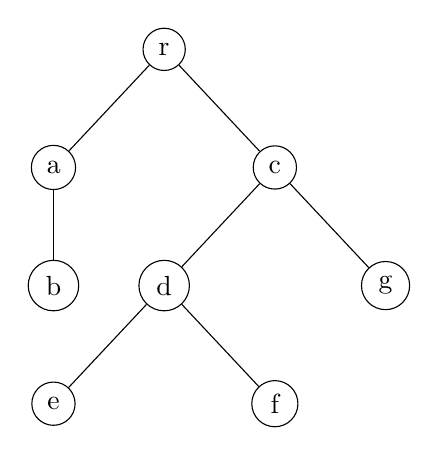
\begin{tikzpicture}[sibling distance=8em,
every node/.style = {shape=circle, draw, align=center}]

\node{r}
	child {node {a}
		child {node {b}}
	}
	child {node {c}
		child {node {d}
			child {node {e}}
			child {node {f}}
		}
		child {node {g}}
	};
\end{tikzpicture}
\end{figure}

\paragraph{Terminologi}~\\
Vi skal se litt på ord og uttrykk for trær. Gjennomgående bruker vi treet i figur \ref{fig:tre} som eksempel

I figuren blir nodene tegnet som rundinger. For å betegne relasjonen mellom nodene bruker vi ofte familierelasjoner. Vi sier at $ e $ og $ f $ er \textbf{søsken}, $ d $ er \textbf{forelder} til $ e $, og $ e $ er \textbf{barn} av $ d $. Vi kan også si at $ g $ er \textbf{onkel} til $ f $, men dette er mindre vanlig, da vi sjeldent har bruk for å snakke om \say{onkelnoder}. 

Nodene $ r, a, c $ og $ d $ kalles \textbf{indre noder}, det vil si at disse nodene har barn. Noder som ikke har noen barn kalles \textbf{løvnoder}

I figur \ref{fig:tre} er $ r $ \textbf{rotnoden}. Rota i treet er den eneste noden uten noen foreldre. Rota er derfor et naturlig startpunkt når vi skal søke eller traversere gjennom treet. 


\subsection{Binære søketrær}
\label{bintraer}
Binære søketrær er trær med noen spesielle krav. Hver node kan ikke ha mer enn to barn, vi kaller dem ofte venstre og høyre barn. Venstre barn er alltid mindre enn noden selv, og høyre barn er alltid større enn noden. Dette gjør binære søketrær meget godt egnet for søking. 

\begin{teorem}
\label{teo:bintre}
Å sette inn, fjerne eller søke etter noder i et binært søketre har
\begin{enumerate}[i]
\item I beste fall $ O(\log n) $ tid
\item I verste fall $ O(n) $ tid
\end{enumerate}
\end{teorem}

Vi skal ikke bevise teorem \ref{teo:bintre} her\footnote{Det kan vises ved induksjon at høyden til et binært tre i beste fall er $ \log_2 n $}, men vi kan se på et eksempel som viser ytterpunktene. I figur \ref{fig:bintre} ser vi to forskjellige binære søketrær. I treet til venstre har vi et fint, balansert tre. Det er lett å se at høyden (og dermed antall operasjoner vi må gjøre for å komme til bunn i treet) er lik $ \lceil \log_2 n \rceil $ der $ n $ er antall noder i treet.

I treet til høyre har hver node kun ett barn. Vi har i praksis en lenkeliste. Hvis vi skal søke etter 4, må vi tråkke gjennom alle de andre nodene for å komme dit. 

\begin{figure}[H]
\caption{To eksempler på binære søketrær}
\label{fig:bintre}
\centering
~\\
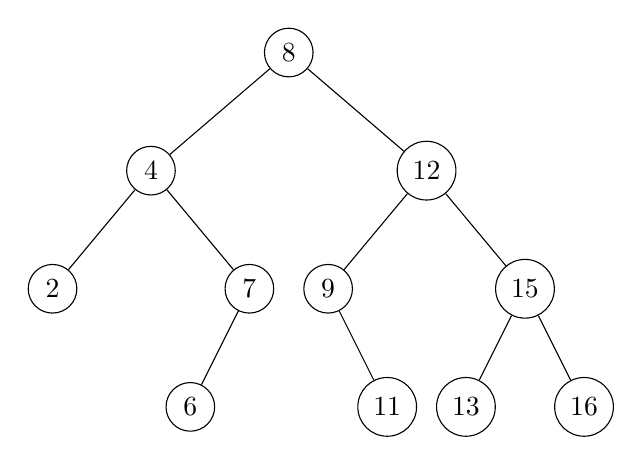
\begin{tikzpicture}[level distance=1.5cm,
  level 1/.style={sibling distance=3.5cm},
  level 2/.style={sibling distance=2.5cm},
  level 3/.style={sibling distance=1.5cm},
every node/.style = {shape=circle, draw, align=center}]

\node{8}
	child {node {4}
		child {node {2}}
		child {node {7}
			child {node {6}}
			child [missing]{}
		}
	}
	child {node {12}
		child {node {9}
			child [missing]{}
			child {node {11}}
		}
		child {node {15}
			child {node {13}}
			child {node {16}}
		}
	};
\end{tikzpicture}
$ \quad\quad $
\begin{tikzpicture}[level distance=1.5cm,sibling distance=2cm,
every node/.style = {shape=circle, draw, align=center}]

\node{1}
	child [missing] {}
	child {node {2}
		child [missing]{}
		child {node {3}
			child [missing]{}
			child {node {4}}
		}
	};
\end{tikzpicture}
\end{figure}




\paragraph{Innsetting}~\\
Når vi skal sette inn en node i et binært søketre starter vi i rota. Vi sammenligner verdien vi skal sette inn med verdien i rota. Hvis verdien vi setter inn er mindre enn rota går vil til venstre, er den større går vi til høyre. Hva som skjer ved likhet er opp til oss å bestemme, men vi må være konsekvente. Når vi kommer til en nullpeker kan vi sette denne pekeren til å peke på noden vi setter inn.

Vi kan implementere denne funksjonen rekursivt. I en ytre klasse kan vi skrive en skallfunksjon som kaller på rotas \verb|instert|-metode. Vi har en indre \verb|Node|-klasse med en rekursiv insertmetode. Den kan implementeres slik:
\javaimport{kode/ex_bintree_insert.java}


\paragraph{Fjerning}~\\
Når vi skal fjerne en node fra et binært søketre har vi tre forskjellige situasjoner som vi må se på.

{\bfseries Noden har ingen barn} (løvnode). Denne situasjonen er ganske grei. Siden noden ikke har noen barn å forholde seg til er det bare å fjerne den fra treet.

{\bfseries Noden har ett barn}. For å fjerne en node $ a $ med ett barn kan vi ganske enkelt flytte pekeren fra foreldernoden til $ a $, til barnet til $ a $.

{\bfseries Noden har to barn}. Hvis noden vi skal fjerne har to barn tar vi opp den minste noden som er større en noden vi skal fjerne og flytter den til den posisjonen noden vi skulle fjærne var. Vi finner den minste noden som er større ved å gå ett steg til høyre, og så til venstre helt til vi er i bunn av treet. 

Eksempel på implementasjon i Java (rekursiv metode i en \verb|Node|-klasse):
\javaimport{kode/ex_bintree_remove.java}


\paragraph{Søking}~\\
Når vi skal søke etter et element i et søketre starter vi i rota og sammenligner det elementet vi søker etter med det elementet som finnes i rota. Er elementet vår mindre enn noden vi ser på går vi til venstre, og er det større går vi til høyre. Deretter foretar vi samme testen på nytt og fortsetter slik til vi enten finner elementet vi leter etter, eller kommer til en nullpeker (bunnen av treet).

Eksempel på implementasjon i Java:
\javaimport{kode/ex_bintree_search.java}





~\\~\\
\subsection{Rød-svarte trær}
Rødsvarte trær er binære søketrær med noen spesielle strukturkrav. Kravene er designet for å motkjempe skjevhet (som illustrert i figur \ref{fig:bintre}), og dermed forbedre kjøretid.

Vi deler nodene opp i to kategorier, røde og svarte. Vi følger noen bestemte regler på hvordan vi skal farge nodene, og fargen på nodene avgjør som vi må benytte oss av rotasjon eller ikke (se \ref{trerotasjon}). Fargen til en node er \textbf{ikke} statisk, den kan endres.

\begin{definisjon}
\label{def:rb_tree}
Et rød-svart tre er et binært søketre der hver node er
farget enten rød eller svart slik at:
\begin{enumerate}[i]
\item Roten er svart.
\item Hvis en node er rød, må barna være svarte.
\item Enhver vei fra en node til en null-peker må inneholde samme antall svarte noder.
\end{enumerate}
\end{definisjon}

Dette sikrer at høyden maksimalt er $ 2\log_2 (n+1) $

\paragraph{Insetting}~\\
For å sette inn en node i rød-svarte trær kan vi bruke algoritmen i teorem \ref{teo:ins_rb}
\begin{teorem} Innsetting i rød-svarte trær. \label{teo:ins_rb}

La $ N $ være noden vi ønsker å sette inn i treet. La $ P $ være forelder, $ G $ besteforelder, og $ U $ onkel til $ N $. Følgende algoritme vil da gi en korrekt innsetting i et rød-svart tre:
\begin{enumerate}
\item Gjør innsetting som i vanlig binært søketre, der $ N $ farges rød.
\item Hvis $ N $ er rota i treet: farg $ N $ svart. 
\item Hvis $ P $ er svart: alt OK. Innsetting ferdig. 
\item Hvis $ P $ er rød og $ N $ ikke er rot:
	\begin{enumerate}
		\item Hvis $ U $ er svart:
		\begin{enumerate}
			\item Farg $ P $ svart
			\item Farg $ G $ rød
			\item Repeter fra pt. 2 med $ G $ som $ N $
		\end{enumerate}
		\item Hvis $ U $ er rød:
		\begin{enumerate}
			\item $ N $ er venstre barn av $ P $, som er venstre barn av $ G $:\\
			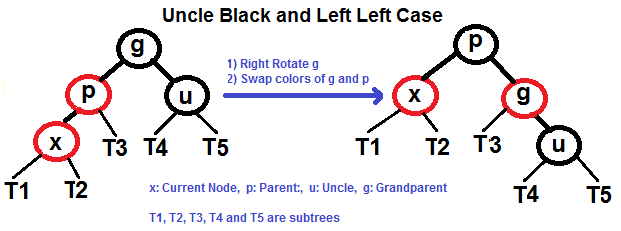
\includegraphics[width=0.65\textwidth]{fig/rbt_ll.png}\\

			\item $ N $ er høyre barn av $ P $, som er venstre barn av $ G $:\\
			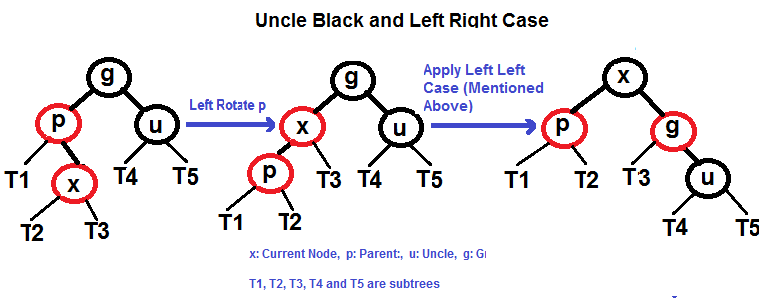
\includegraphics[width=0.65\textwidth]{fig/rbt_lr.png}\\
			
			\item $ N $ er høyre barn av $ P $, som er høyre barn av $ G $ (speilvendt av i):\\
			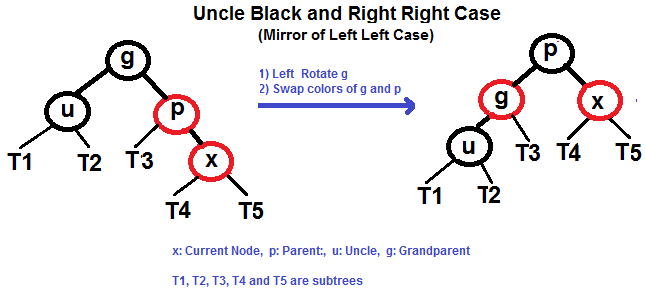
\includegraphics[width=0.65\textwidth]{fig/rbt_rr.png}\\
			
			\item $ N $ er venstre barn av $ P $, som er høyre barn av $ G $ (speilvendt av ii):\\
			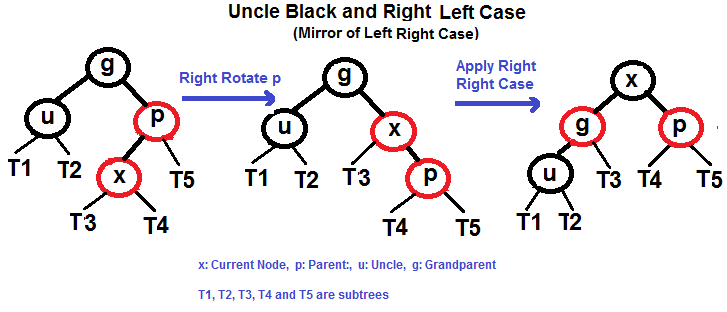
\includegraphics[width=0.65\textwidth]{fig/rbt_rl.png}\\
			
		\end{enumerate}
	\end{enumerate}
\end{enumerate}
\end{teorem}


\paragraph{Fjerning}~\\
Vi skal fjerne en node $ N $ fra et rød-svart tre.

Vi ser på noen spesialtifeller: Hvis $ N $ er en rød node er jobben enkel. Vi sletter da $ N $ som om vi hadde et vanlig søketre. Det samme gjelder hvis forelderen til $ N $ er rød og $ N $ er eneste barn. Hvis $ N $ er svart og har ett barn sletter vi $ N $ og farger barnet svart. 

Generelt sletter vi noden som i et vanlig binært søketre, og utfører nødvendige rotasjoner og omfarginger for å beholde kravet i definisjon \ref{def:rb_tree}.


\paragraph{Tidsanalyse}~\\
Siden høyden til et rød-svart tre maksimalt er $ 2\log_2 (n+1) $ har vi worst case tid $ O(\log_2 n) $. Selv om vi risikerer å måtte gjøre rotasjoner er innsetningstiden også $ O(\log_2 n) $.


~\\
\subsection{B-trær}
B-trær er konstruert for å effektivisere antall disklesninger, og gir mening å bruke hvis vi har et tre som er så stort at det må lagres på gammeldagse spinnedisker, og ikke i RAM. Vi lagrer dataene i blokker, og leser en og en blokk av gangen. Alle dataene er lagret i løvnodene, mens de indre nodene brukes for søking. En vanlig måte å implementere B-trær på er å ha så mye av toppen i RAM som mulig, og lagre resten på disk. B-trær er ikke binære, dvs at de kan ha flere enn 2 barn. 

\begin{definisjon} La $ M $ angi antall mulige nøkler i hver indre node, og $ L $ angi maksimalt antall dataelementer i hver løvnode. B-trær er søketrær der følgende kriterier er oppfylt:
\begin{enumerate}[i]
\item Alle dataene er lagret i løvnodene
\item Interne noder lagrer inntil $ M-1 $ nøkler for søking: nøkkel $ i $ angir den minste verdien i subtre $ i+1 $.
\item Roten er enten en løvnode, eller har mellom 2 og $ M $ barn. 
\item Alle andre indre noder har mellom $ \lceil M/2\rceil $ og $ M $ barn. 
\item Alle løvnoder har samme dybde.
\item Alle løvnoder har mellom $ \lceil L/2\rceil $ og $ L $ dataelementer
\end{enumerate}
\label{def:b_tre}
\end{definisjon}


\paragraph{Innsetting}~\\
Når vi skal sette inn et element i et B-tre finner vi plassen elementet skal på, og setter det der. Hvis løvnoden vi setter elementet inn i er full må vi splitte noden i to like store deler. Vi må da oppdatere nøklene i foreldrenoden $ P $. Hvis $ P $ ikke har plass til en ekstra nøkkel må vi splitte den også, og oppdatere nøklene i foreldrenoden til $ P $. Slik fortsetter vi oppover til vi får en node som har plass til en ekstra nøkkel. Den eneste måten et B-tre kan øke høyden på er at rota splittes i to, og at vi lager en ny rot. 

\begin{eks} Sett inn 13 og 42 i følgende B-tre ($ M = 3 $ og $ N = 4 $):
\begin{figure}[H]
\centering
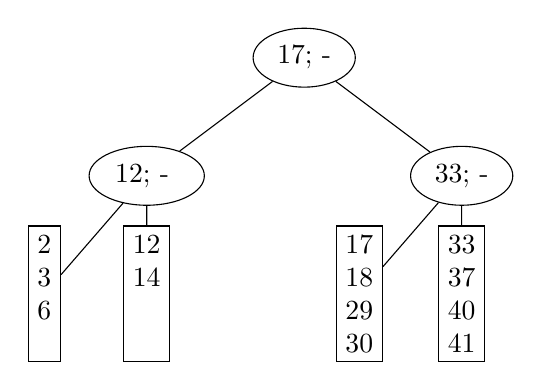
\begin{tikzpicture}
[level distance=1.5cm,
  level 1/.style={sibling distance=4cm},
  level 2/.style={sibling distance=1.3cm},
every node/.style = {align=center}]
\tikzstyle{inner} = [ellipse, draw=black]
\tikzstyle{leaf} = [rectangle, draw=black]

\node[inner] {17; -}
child {
	node[inner] {12; - }
	child {
		node[leaf] {2\\3\\6\\~}
	}
	child {
		node[leaf] {12\\14\\~\\~}
	}
	child[missing]
}
child {
	node[inner] {33; -}
	child {
		node[leaf] {17\\18\\29\\30}
	}
	child {
		node[leaf] {33\\37\\40\\41}
	}
	child[missing]
}
;

\end{tikzpicture}
\end{figure}

Vi starter med å sette inn 13. Vi ser først på rota: (17; -). 13 er mindre enn 17, så vi går til første barn. Så sammenligner vi med (12; -). 13 er sørre enn 13, og mindre enn uendelig (- symboliserer minste verdi i tredje barn, men siden det barnet ikke eksisterer tenker vi på verdier som $ \infty $). Vi går derfor til andre barn. Der ser vi at vi kan sette inn 13 uten problemer. 

Vi skal nå sette inn 42. 42 er større enn 33 så vi går til andre barn. Igjen er 42 større enn 33 så vi går til andre barn igjen. Her ser vi at hvis vi legger til 42 i bunn av noden (33, 37, 40, 41) blir størrelsen lik 5, altså større enn $ N $. Vi må splitte noden. Når vi splitter en node med et odde antall elementer er det ikke helt klart som vi skal ta med oss størsteparten, eller la størsteparten være igjen. I dette tilfellet vil vi få en node med 3 og en node med 2 elementer. Vi kan selv velge om den nye noden skal ha 2 eller 3 elementer, men vi må være konsekvente. I dette tilfellet lar vi den nye noden ha 2 elementer. Vi oppdaterer foreldrenoden. Siden den har to barn fra før og $ M=3 $ går det fint, vi trenger ikke splitte videre oppover. 

Resultatet etter innsetting ser slik ut:

\begin{figure}[H]
\centering
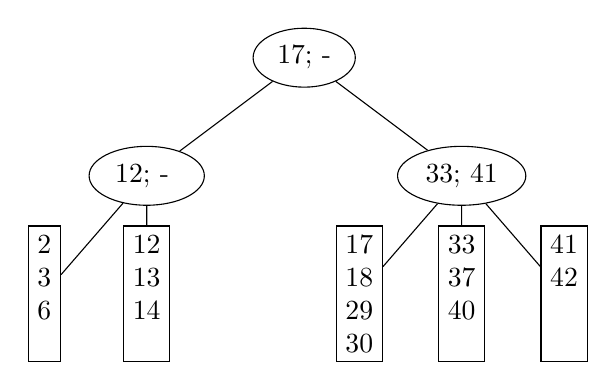
\begin{tikzpicture}
[level distance=1.5cm,
  level 1/.style={sibling distance=4cm},
  level 2/.style={sibling distance=1.3cm},
every node/.style = {align=center}]
\tikzstyle{inner} = [ellipse, draw=black]
\tikzstyle{leaf} = [rectangle, draw=black]

\node[inner] {17; -}
child {
	node[inner] {12; - }
	child {
		node[leaf] {2\\3\\6\\~}
	}
	child {
		node[leaf] {12\\13\\14\\~}
	}
	child[missing]
}
child {
	node[inner] {33; 41}
	child {
		node[leaf] {17\\18\\29\\30}
	}
	child {
		node[leaf] {33\\37\\40\\~}
	}
	child {
		node[leaf] {41\\42\\~\\~}
	}
}
;

\end{tikzpicture}
\end{figure}
\end{eks}

~\\
\paragraph{Fjerning}~\\
Hvis vi skal fjerne et element fra et B-tre søker vi opp elementet, tar det vekk, og hvis mengden elementer i noden blir mindre enn grensen satt i def. \ref{def:b_tre}.vi slår vi sammen to noder. Den eneste måten B-trær kan minke i høyde på er om alle barna til rota blir slått sammen til én node (vi fjerner da rota). 

\begin{eks} Fjern 41 fra følgende B-tre:

\begin{figure}[H]
\centering
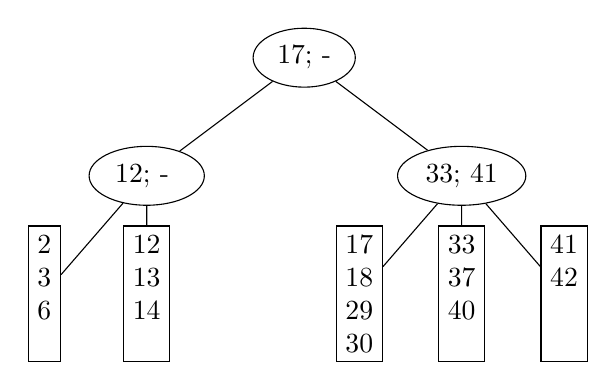
\begin{tikzpicture}
[level distance=1.5cm,
  level 1/.style={sibling distance=4cm},
  level 2/.style={sibling distance=1.3cm},
every node/.style = {align=center}]
\tikzstyle{inner} = [ellipse, draw=black]
\tikzstyle{leaf} = [rectangle, draw=black]

\node[inner] {17; -}
child {
	node[inner] {12; - }
	child {
		node[leaf] {2\\3\\6\\~}
	}
	child {
		node[leaf] {12\\13\\14\\~}
	}
	child[missing]
}
child {
	node[inner] {33; 41}
	child {
		node[leaf] {17\\18\\29\\30}
	}
	child {
		node[leaf] {33\\37\\40\\~}
	}
	child {
		node[leaf] {41\\42\\~\\~}
	}
}
;

\end{tikzpicture}
\end{figure}
Vi ser at 41 er mellom 17 og $ \infty $, så vi går til andre barn. Deretter ser vi at 41 er større enn 33 og større enn eller lik 41. Vi går derfor til tredje barn og fjerner 41. Vi ser at da vi noden kun ha ett element, og vi slår den sammen med noden før. Resultatet etter fjerning blir
\begin{figure}[H]
\centering
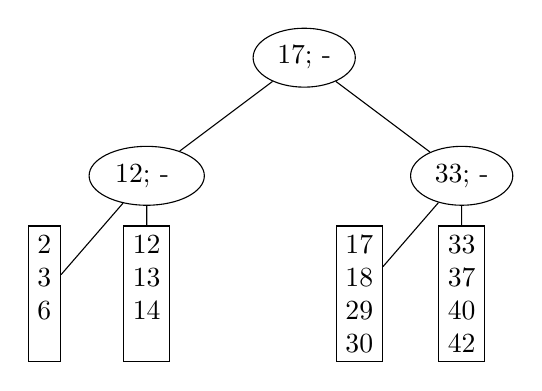
\begin{tikzpicture}
[level distance=1.5cm,
  level 1/.style={sibling distance=4cm},
  level 2/.style={sibling distance=1.3cm},
every node/.style = {align=center}]
\tikzstyle{inner} = [ellipse, draw=black]
\tikzstyle{leaf} = [rectangle, draw=black]

\node[inner] {17; -}
child {
	node[inner] {12; - }
	child {
		node[leaf] {2\\3\\6\\~}
	}
	child {
		node[leaf] {12\\13\\14\\~}
	}
	child[missing]
}
child {
	node[inner] {33; -}
	child {
		node[leaf] {17\\18\\29\\30}
	}
	child {
		node[leaf] {33\\37\\40\\42}
	}
	child[missing]
}
;

\end{tikzpicture}
\end{figure}
\end{eks}



\paragraph{Tidsanalyse}

\begin{teorem} Å søke etter, sette inn og fjerne elementer fra et B-tre tar, både i beste og verste fall, $ O(\log n) $ tid.
\end{teorem}




\newpage
\subsection{Rotasjon}
\label{trerotasjon}

\subsubsection{Zig}
For å skjønne zig-rotasjon ser vi på en figur:

\begin{figure}[H]
\caption{Zig-rotasjon mhp X}
\centering
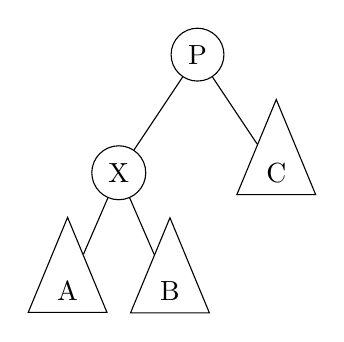
\begin{tikzpicture}[level distance=1.5cm,
  level 1/.style={sibling distance=2cm},
  level 2/.style={sibling distance=1.3cm}]

\tikzstyle{subtree} = [isosceles triangle, draw=black, align=center, minimum height=0.5cm, minimum width=1cm, shape border rotate=90, anchor=center]
\tikzstyle{n} = [draw=black, draw=black, align=center, circle]

\node[n] {P}
child {
	node[n] {X}
	child {
		node[subtree] {A}
	}
	child {
		node[subtree] {B}
	}
}
child {
	node[subtree] {C}
}
;
\end{tikzpicture}
\quad\raisebox{5\height}{\scalebox{2}{$\rightarrow$}}\quad
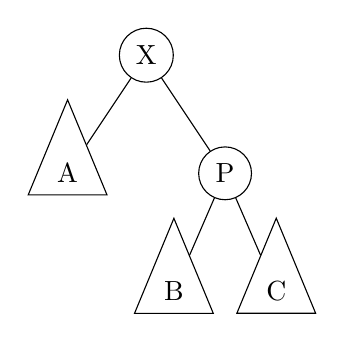
\begin{tikzpicture}[level distance=1.5cm,
  level 1/.style={sibling distance=2cm},
  level 2/.style={sibling distance=1.3cm}]

\tikzstyle{subtree} = [isosceles triangle, draw=black, align=center, minimum height=0.5cm, minimum width=1cm, shape border rotate=90, anchor=center]
\tikzstyle{n} = [draw=black, draw=black, align=center, circle]

\node[n] {X}
child {
	node[subtree] {A}
}
child {
	node[n] {P}
	child {
		node[subtree] {B}
	}
	child {
		node[subtree] {C}
	}
}
;
\end{tikzpicture}
\end{figure}

En zig-rotasjon vil beholde egenskapene til et binært søketre siden alle nodene i A er mindre enn X og P, alle nodene i B er større enn X og mindre enn P, og alle nodene i C er større enn både X og P. Vi ser at alle høyre barn av P også er høyre barn av P \emph{etter} rotasjonen, etc. 

Vi har også noe som heter zig-zig-rotasjon, som er å utføre en zig-rotasjon to ganger.


\subsubsection{Zig-zag}
Igjen ser vi på en figur:

\begin{figure}[H]

% Dette er helt forferdelig kode. Jeg vet, og jeg beklager. 

\caption{Zig-zag-rotasjon mhp X:}
\centering
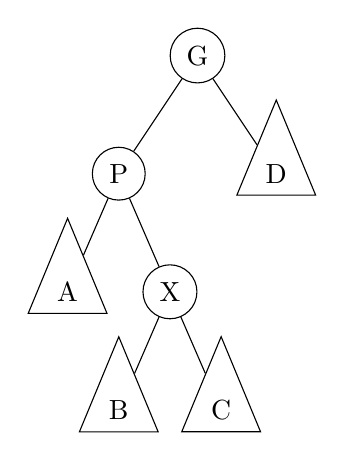
\begin{tikzpicture}[level distance=1.5cm,
  level 1/.style={sibling distance=2cm},
  level 2/.style={sibling distance=1.3cm}]

\tikzstyle{subtree} = [isosceles triangle, draw=black, align=center, minimum height=0.5cm, minimum width=1cm, shape border rotate=90, anchor=center]
\tikzstyle{n} = [draw=black, draw=black, align=center, circle]

\node[n] {G}
child {
	node[n] {P}
	child {
		node[subtree] {A}
	}
	child {
		node[n] {X}
		child {
			node[subtree] {B}
		}
		child {
			node[subtree] {C}
		}
	}
}
child {
	node[subtree] {D}
}
;
\end{tikzpicture}
\quad\raisebox{9\height}{\scalebox{2}{$\rightarrow$}}\quad
\raisebox{.25\height}{
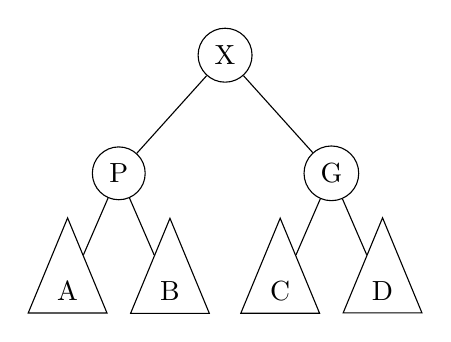
\begin{tikzpicture}[level distance=1.5cm,
  level 1/.style={sibling distance=2.7cm},
  level 2/.style={sibling distance=1.3cm}]

\tikzstyle{subtree} = [isosceles triangle, draw=black, align=center, minimum height=0.5cm, minimum width=1cm, shape border rotate=90, anchor=center]
\tikzstyle{n} = [draw=black, draw=black, align=center, circle]

\node[n] {X}
child {
	node[n] {P}
	child {
		node[subtree] {A}
	}
	child {
		node[subtree] {B}
	}
}
child {
	node[n] {G}
	child {
		node[subtree] {C}
	}
	child {
		node[subtree] {D}
	}
}
;
\end{tikzpicture}
}
\end{figure}

Som i tilfellet med zig-rotasjon ser vi at egenskapene til et binært søketre er bevart. 				% ferdig, mangler indexer
\newpage
\section{Grafer}
En graf er en samling av kanter og noder. Vi kaller mengden av alle nodene $ V $ (verticies), og mengden av alle kantene $ E $ (edges). Grafen $ G $ blir da en samling av disse to mengdene. Formelt kan vi definere en graf slik: \index{graf}

\begin{definisjon}
En graf $ G $  er et par $ (V, E) $, der $ V $ er en ikke-tom mengde noder og $ E $ en mengde nodepar $ \{v_1, v_2\} $; $ v_1, v_2 \in V $ der $ \{v_1, v_2\} $ angir at grafen inneholder en kant fra $ v_1 $ til $ v_2 $.
\end{definisjon}


\paragraph{Terminologi}~\\
Vi bruker $ |E| $ for å betegne antall kanter og $ |V| $ for å betegne antall noder. \index{graf!kant}\index{graf!node}\index{node!graf}

Vi sier at en node er \textbf{nabo} med en annen node hvis de har en kant mellom seg. I figur \ref{fig:graf} er B og A naboer, men A og C er ikke naboer. \index{graf!nabo}

En \textbf{sti} eller \textbf{vei} er en sekvens av noder (og kantene mellom dem) fra en node til en annen. En sti fra A til G i figuren under kan for eksempel være A, D, C, G. (siden grafen inneholder løkker er ikke stien entydig) \index{graf!sti}\index{graf!vei}

En graf er \textbf{rettet} hvis kantene har en spesiell retning, og \textbf{urettet} hvis vi ikke bryr oss om retningen på kantene. I en rettet graf vil kanten $ \{v_1, v_2\} $ bety at det går en kant fra $ v_1 $ til $ v_2 $, men ikke nødvendigvis fra $ v_2 $ til $ v_1 $. Grafen i figur \ref{fig:tre} er urettet. Hvis en graf er rettet kaller vi ofte naboene for \textbf{etterfølgere}.  \index{graf!rettet}\index{graf!urettet}

En graf er \textbf{vektet} hvis kantene har en verdi knyttet til seg, ofte kalt \emph{kosten} til kanten. I en \textbf{uvektet} graf har ikke kantene noen spesiell verdi. Vi kan tenke på en uvektet graf som en vektet graf der alle kantene har kost = 1. \index{graf!vektet}\index{graf!uvektet}

Grafen er \textbf{syklisk} hvis den inneholder løkker, og \textbf{asyklisk} hvis den ikke inneholder løkker. I figur \ref{fig:graf} ser vi at A, B, C, D danner en løkke (det gjør også C, G, F, E). Grafen er derfor syklisk.\index{graf!syklisk}\index{graf!asyklisk}

En type grafer vi jobber mye med er \textbf{DAG}er. DAG står for \emph{Directed Asyclic Graph}, på norsk: en rettet, asyklisk graf. \index{graf!DAG}


\begin{figure}[H]
\centering
\caption{Eksempel på en urettet, uvektet graf}~\\
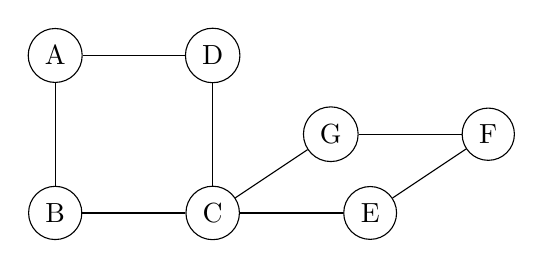
\begin{tikzpicture}
\tikzstyle{vertex} = [circle, draw=black]
\tikzstyle{edge} = [draw=black]

\node[vertex] (A) at (-1,0) {A};
\node[vertex] (B) at (-1,-2) {B};
\node[vertex] (C) at (1,-2) {C};
\node[vertex] (D) at (1,0) {D};
\node[vertex] (E) at (3,-2) {E};
\node[vertex] (F) at (4.5,-1) {F};
\node[vertex] (G) at (2.5, -1) {G};

\draw[edge] (B) -- (A);
\draw[edge] (B) -- (C);
\draw[edge] (A) -- (D);
\draw[edge] (C) -- (E);
\draw[edge] (C) -- (D);
\draw[edge] (E) -- (F);
\draw[edge] (C) -- (G);
\draw[edge] (G) -- (F);
\end{tikzpicture}
\label{fig:graf}
\end{figure}


\subsection{Begreper}

\subsubsection{Hamiltonsk sti}
En hamiltonsk sti er en sti som besøker alle nodene én gang. Dette kan virke som en triviell sak, men i en del tilfeller er det faktisk ikke mulig å finne en hamiltonsk sti. I grafen i figur \ref{fig:graf} er B, A, D, C, G, F, E en hamiltonsk sti (det finnes fler). \index{hamiltonsk sti} \index{graf!hamiltonsk sti}

Et berømt eksempel på en graf \emph{uten} en hamiltonsk sti er broene i Königsberg: \index{broene i Königsberg}
\begin{figure}[H]
\centering
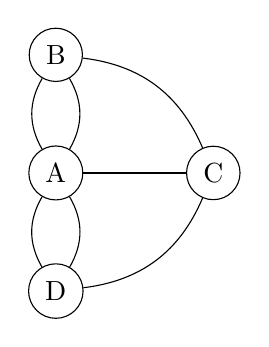
\begin{tikzpicture}
\tikzstyle{vertex} = [circle, draw=black]
\tikzstyle{edge} = [draw=black]

\node[vertex] (A) at (0,0) {A};
\node[vertex] (B) at (0,1.5) {B};
\node[vertex] (C) at (2,0) {C};
\node[vertex] (D) at (0, -1.5) {D};

\draw[edge] (A) to (C);
\draw[edge] (B) to [bend left] (C);
\draw[edge] (A) to [bend left] (B);
\draw[edge] (A) to [bend right] (B);
\draw[edge] (A) to [bend left] (D);
\draw[edge] (A) to [bend right] (D);
\draw[edge] (D) to [bend right] (C);
\end{tikzpicture}
\end{figure}



\subsubsection{Spenntrær}
Vi begynner med en definisjon:\index{spenntre} \index{minimalt spenntre}

\begin{definisjon}
Et \textbf{spenntre} for en urettet graf $ G $ er et tre med kanter fra grafen slik at alle nodene i $ G $ er forbundet. Spesielt er et \textbf{minimalt spenntre} de(t) spenntre(ene) med lavest total kostnad.
\end{definisjon}

\noindent Minimale spenntrær er sjeldent entydig bestemt. Vi har et entydig minimalt spenntre hvis alle kantene har forskjellig vekt. Vi tegner opp et eksempel:

\begin{figure}[H]
\centering
\caption{En graf (venstre) og et minimalt spenntre for grafen (høyre)}~\\
\label{fig:min_spenntre}
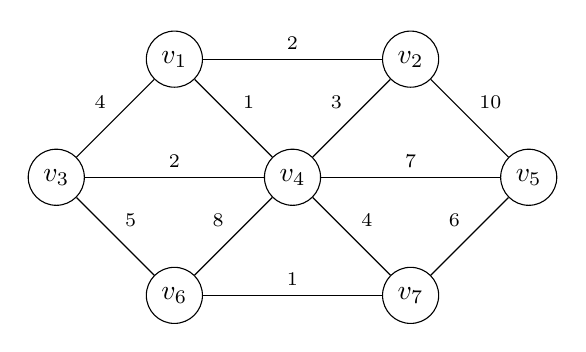
\begin{tikzpicture}[auto,node distance=2cm]
\tikzstyle{vertex} = [circle, draw=black]
\tikzstyle{edge} = [draw=black]

\node[vertex] (v1) at (-1.5,1.5) {$ v_1 $};
\node[vertex] (v2) at (1.5, 1.5) {$ v_2 $};
\node[vertex] (v3) at (-3,0) {$ v_3 $};
\node[vertex] (v4) at (0,0) {$ v_4 $};
\node[vertex] (v5) at (3,0) {$ v_5 $};
\node[vertex] (v6) at (-1.5,-1.5) {$ v_6 $};
\node[vertex] (v7) at (1.5,-1.5) {$ v_7 $};

\draw[edge] (v3) to node{\scriptsize4} (v1);
\draw[edge] (v3) to node{\scriptsize2} (v4);
\draw[edge] (v3) to node{\scriptsize5} (v6);
\draw[edge] (v1) to node{\scriptsize1} (v4);
\draw[edge] (v6) to node{\scriptsize8} (v4);
\draw[edge] (v4) to node{\scriptsize3} (v2);
\draw[edge] (v4) to node{\scriptsize4} (v7);
\draw[edge] (v4) to node{\scriptsize7} (v5);
\draw[edge] (v2) to node{\scriptsize10} (v5);
\draw[edge] (v7) to node{\scriptsize6} (v5);
\draw[edge] (v1) to node{\scriptsize2} (v2);
\draw[edge] (v6) to node{\scriptsize1} (v7);
\end{tikzpicture}~~
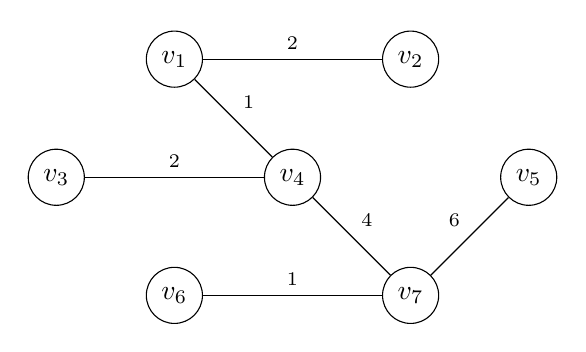
\begin{tikzpicture}[auto,node distance=2cm]
\tikzstyle{vertex} = [circle, draw=black]
\tikzstyle{edge} = [draw=black]

\node[vertex] (v1) at (-1.5,1.5) {$ v_1 $};
\node[vertex] (v2) at (1.5, 1.5) {$ v_2 $};
\node[vertex] (v3) at (-3,0) {$ v_3 $};
\node[vertex] (v4) at (0,0) {$ v_4 $};
\node[vertex] (v5) at (3,0) {$ v_5 $};
\node[vertex] (v6) at (-1.5,-1.5) {$ v_6 $};
\node[vertex] (v7) at (1.5,-1.5) {$ v_7 $};

\draw[edge] (v3) to node{\scriptsize2} (v4);
\draw[edge] (v1) to node{\scriptsize1} (v4);
\draw[edge] (v4) to node{\scriptsize4} (v7);
\draw[edge] (v7) to node{\scriptsize6} (v5);
\draw[edge] (v1) to node{\scriptsize2} (v2);
\draw[edge] (v6) to node{\scriptsize1} (v7);
\end{tikzpicture}~\\~\\
\end{figure}

For å finne et minimalt spenntre til en graf kan vi bruke Prims algoritme (\ref{prim}) eller Kruskals algoritme (\ref{kruskal})


\subsubsection{Topologisk sortering}
Topologisk sortering er en ordning av noder i en DAG slik at dersom det finnes en vei fra $ v_i $ til $ v_j $ i grafen kommer $ v_i $ før $ v_j $ i sorteringa. En topologisk sortering er ikke nødvendigvis entydig bestemt, ofte finnes det veldig mange. Hvis en graf er syklisk eksisterer det ikke en topologisk sortering av grafen. Vi ser på et eksempel: \index{topologisk sortering}

\begin{eks} Gitt følgende graf, finn alle topologiske sorteringer.
\begin{figure}[H]
\centering
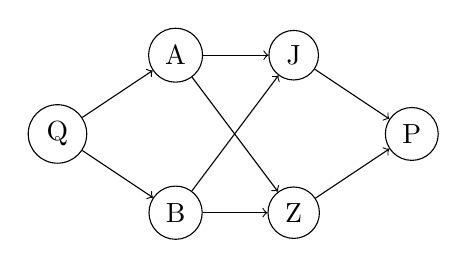
\begin{tikzpicture}[->]
\tikzstyle{v} = [circle, draw=black]
\tikzstyle{e} = [draw=black]

\node[v] (Q) at (-3, 0) {Q};
\node[v] (A) at (-1.5, 1) {A};
\node[v] (B) at (-1.5, -1) {B};
\node[v] (J) at (0, 1) {J};
\node[v] (Z) at (0, -1) {Z};
\node[v] (P) at (1.5, 0) {P};

\draw[e] (Q) to (A);
\draw[e] (Q) to (B);
\draw[e] (A) to (J);
\draw[e] (B) to (Z);
\draw[e] (B) to (J);
\draw[e] (A) to (Z);
\draw[e] (J) to (P);
\draw[e] (Z) to (P);
\end{tikzpicture}
\end{figure}

Vi ser at Q har inngrad 0, det er derfor et logisk sted å begynne. Etter Q kommer A og B. Vi ser at vi kan ikke gå videre fra A før uten å ha vært innom B, siden både J og Z er avhengige av B. Tilsvarende kan vi ikke gå videre fra B før vi har vært innom A. Til slutt ser vi at P er avhengig av både J og Z. Begge de to må derfor komme før P i sorteringa. Vi har da dekt alle mulige utfall. Vi kan liste opp alle mulige sorteringer:
\begin{itemize}
\item Q, A, B, J, Z, P
\item Q, B, A, J, Z, P
\item Q, A, B, Z, J, P
\item Q, B, A, Z, J, P
\end{itemize}

Vi kan ta med et moteksempel også: Q, A, J, B, Z, P er ikke en gyldig topologisk sortering siden J kommer før B i sorteringa, men i grafen ser vi at J er avhengig av B (det går en kant fra B til J).
\end{eks}



\subsubsection{Strongly connected components (SCC)}
Vi ser på definisjonen av strongly connected components (heretter SCC): \index{SCC (strongly connected components)}
\begin{definisjon}
Anta at vi har en rettet graf $ G = (V, E) $. Vi har da at en \textbf{SCC} av $ G $ er et maksimalt sett av noder $ U \subseteq V $ slik at for alle $ u_i $, $ u_j \in U $ har vi at $ u_i \leadsto u_j $ og $ u_j \leadsto u_i $.
\end{definisjon}

Med andre ord: en SCC er en del (partisjon) av grafen der alle nodene i den partisjonen kan nå alle andre noder i partisjonen. Vi ser på et eksempel: \index{graf!partisjon}

\begin{eks} Finn alle SCCer i grafen:
\begin{figure}[H]
\centering
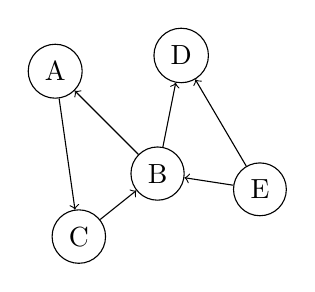
\begin{tikzpicture}[->]
\tikzstyle{v} = [circle, draw=black]
\tikzstyle{e} = [draw=black]

\node[v] (A) at (-1.3, 1.3) {A};
\node[v] (B) at (0, 0) {B};
\node[v] (C) at (-1, -.8) {C};
\node[v] (D) at (0.3, 1.5) {D};
\node[v] (E) at (1.3, -0.2) {E};

\draw[e] (A) to (C);
\draw[e] (C) to (B);
\draw[e] (B) to (A);
\draw[e] (B) to (D);
\draw[e] (E) to (B);
\draw[e] (E) to (D);
\end{tikzpicture}
\end{figure}
Vi ser at \{A, B, C\} danner en SCC. D har ingen kanter ut. Den må derfor være sin egen SCC. E ingen kanter inn, den må også være sin egen SCC. Vi har da at vi kan partisjonere grafen slik: \{\{A, B, C\}, \{D\}, \{E\} \}
\end{eks}

\subsubsection{Articulation points og biconnectivity}
Et \textbf{articulation point} er et kritisk punkt i en sammenhengende graf som ikke kan fjernes uten at grafen ikke lenger er sammenhengende. I grafen i figur \ref{fig:graf} er C et slikt punkt. Vi ser at vi kan ta vekk A uten noen store komplikasjoner, men hvis vi tar vekk C vil ikke lenger B og E være sammenknyttet.\index{graf!articulation points}

En \textbf{biconnected} graf er en graf uten articulation points, altså en graf der det alltid finnes mer enn én vei fra en node til en annen. Grafen (til venstre) i figur \ref{fig:min_spenntre} er en slik graf. \index{graf!biconnected}

\subsection{Grafalgoritmer}

\subsubsection{Dybde først}
\label{dfs}
Dybde-først-traversering (herfra dfs: depth first search) er en måte å traversere gjennom en graf på. Det kan tenkes på som en generalisering av dybde-først-traversering gjennom trær. Vi velger oss en (hvilken som helst) startnode, og beveger oss ned til etterfølgerne til noden. Når vi kommer til en node som ikke har kanter til en ubesøkt node (enten at noden har utgrad 0, eller at alle etterfølgerne er besøkt) går vi tilbake. 

Underveis i traverseringen har vi en teller som holder styr på hvor mange skritt vi har tatt. I hver node lagrer vi verdien av telleren prefix og postfix, det vil si første gang vi kommer til noden og når vi kommer tilbake etter å ha vært nedom barna. 

\begin{figure}[H]
\centering
\captionsetup{justification=centering,margin=1cm}
\caption{En rettet graf med tallene lagret etter et dfs. Heltrukne linjer er kanter vi besøkte i dfs-et, striplede linjer er kanter vi ikke besøkte}~\\
\label{fig:dfs}
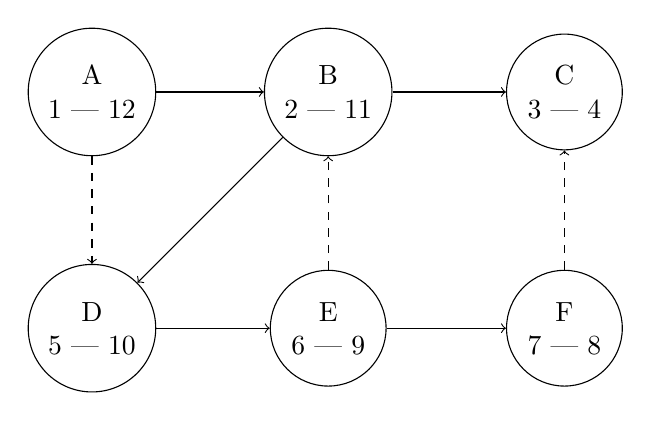
\begin{tikzpicture}[->, align=center]
\tikzstyle{v} = [circle, draw=black]
\tikzstyle{e} = [draw=black]
\tikzstyle{eh} = [draw=black, dashed]

\node[v](A) at (0, 3) {A\\1 | 12};
\node[v](B) at (3, 3) {B\\2 | 11};
\node[v](C) at (6, 3) {C\\3 | 4};
\node[v](D) at (0, 0) {D\\5 | 10};
\node[v](E) at (3, 0) {E\\6 | 9};
\node[v](F) at (6, 0) {F\\7 | 8};

\draw[e] (A) to (B);
\draw[e] (B) to (D);
\draw[eh] (A) to (D);
\draw[e] (D) to (E);
\draw[e] (E) to (F);
\draw[eh] (F) to (C);
\draw[e] (B) to (C);
\draw[eh] (E) to (B);
\end{tikzpicture}
\end{figure}

I figur \ref{fig:dfs} har vi brukt A som rotnode. Vi gikk deretter til et av barna, B. Videre gikk vi til C, og siden C har utgrad 0 måtte vi gå tilbake til B igjen. Fra B gikk vi videre til D, så til E og til F. Fra F går det en kant til C, men siden vi har besøkt C fra før går vi tilbake igjen. 

DFS-algorigmer er velegnet for å programmere rekursivt. Et eksempel på en enkel implementasjon i Java (som en metode i en Node-klasse):

\javaimport{kode/dfs.java}
\newpage

\subsubsection{Kosarajus algoritme (Finne SCC)}
Vi kan finne SCCer i en graf $ G $ ved å utføre to dfs. Et på $ G $ og et på $ G^t $, som er grafen vi får ved å snu alle kantene i $ G $. Denne algoritmen kalles Kosarajus algoritme.

\begin{teorem} Kosarajus algoritme

La $ G $ være en rettet graf. Utfør et dfs på $ G $ fra en hvilken som helst startnode, og lagre postfix-telleren (det som ble kalt \verb|highNum| i kodeekempelet i \ref{dfs}). Hvis søket slutter før alle nodene er besøkt, starter vi fra en ny, ubesøkt node.

Snu alle kantene i (transponer) $ G $ og dann $ G^t $. Sorter nodene i $ G $ synkende etter verdien på postfix-telleren. Start et dfs i $ G^t $ fra den noden som har høyest verdi. Alle nodene vi da besøker danner en SCC. Fjern så alle nodene vi besøkte fra grafen $ G^t $, og utfør et nytt dfs fra den noden som nå har høyest tellerverdi. Fortsett slik til alle nodene er besøkt. 
\end{teorem}


\noindent Vi ser på et eksempel:

\begin{eks} Finn alle SCCer i grafen:

\begin{figure}[H]
\centering
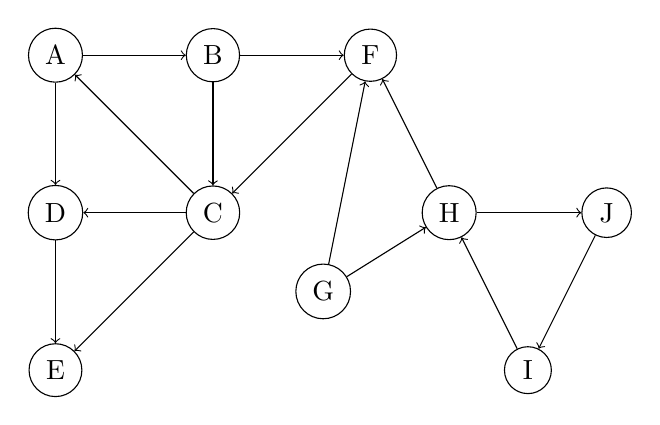
\begin{tikzpicture}[->, align=center]
\tikzstyle{v} = [circle, draw=black]
\tikzstyle{e} = [draw=black]

\node[v] (A) at (-2, 2) {A};
\node[v] (B) at (0, 2) {B};
\node[v] (C) at (0, 0) {C};
\node[v] (D) at (-2, 0) {D};
\node[v] (E) at (-2, -2) {E};
\node[v] (F) at (2, 2) {F};
\node[v] (G) at (1.4, -1) {G};
\node[v] (H) at (3, 0) {H};
\node[v] (I) at (4, -2) {I};
\node[v] (J) at (5, 0) {J};

\draw[e] (A) to (B);
\draw[e] (A) to (D);
\draw[e] (B) to (C);
\draw[e] (B) to (F);
\draw[e] (C) to (A);
\draw[e] (C) to (D);
\draw[e] (C) to (E);
\draw[e] (D) to (E);
\draw[e] (F) to (C);
\draw[e] (G) to (F);
\draw[e] (G) to (H);
\draw[e] (H) to (F);
\draw[e] (H) to (J);
\draw[e] (I) to (H);
\draw[e] (J) to (I);
\end{tikzpicture}
\end{figure}

Vi begynner med å gjøre et dfs. Vi starter i A. Søket stopper etter å ha besøkt A, B, C, D, E og F, og må starte på nytt i G. Startpunktene er valg tilfeldig, og kunne like gjerne vært noen andre. 

\begin{figure}[H]
\centering
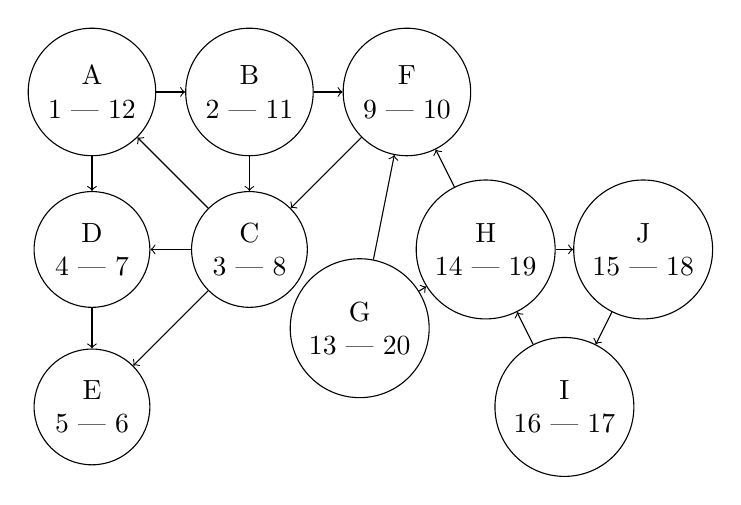
\begin{tikzpicture}[->, align=center]
\tikzstyle{v} = [circle, draw=black]
\tikzstyle{e} = [draw=black]

\node[v] (A) at (-2, 2) {A\\1 | 12};
\node[v] (B) at (0, 2) {B\\2 | 11};
\node[v] (C) at (0, 0) {C\\3 | 8};
\node[v] (D) at (-2, 0) {D\\4 | 7};
\node[v] (E) at (-2, -2) {E\\5 | 6};
\node[v] (F) at (2, 2) {F\\9 | 10};
\node[v] (G) at (1.4, -1) {G\\13 | 20};
\node[v] (H) at (3, 0) {H\\14 | 19};
\node[v] (I) at (4, -2) {I\\16 | 17};
\node[v] (J) at (5, 0) {J\\15 | 18};

\draw[e] (A) to (B);
\draw[e] (A) to (D);
\draw[e] (B) to (C);
\draw[e] (B) to (F);
\draw[e] (C) to (A);
\draw[e] (C) to (D);
\draw[e] (C) to (E);
\draw[e] (D) to (E);
\draw[e] (F) to (C);
\draw[e] (G) to (F);
\draw[e] (G) to (H);
\draw[e] (H) to (F);
\draw[e] (H) to (J);
\draw[e] (I) to (H);
\draw[e] (J) to (I);
\end{tikzpicture}
\end{figure}

\noindent Det hadde vært nok å bare lagre postfixverdiene, men vi har tatt med begge for oversiktens skyld. Vi transponerer $ G $:

\begin{figure}[H]
\centering
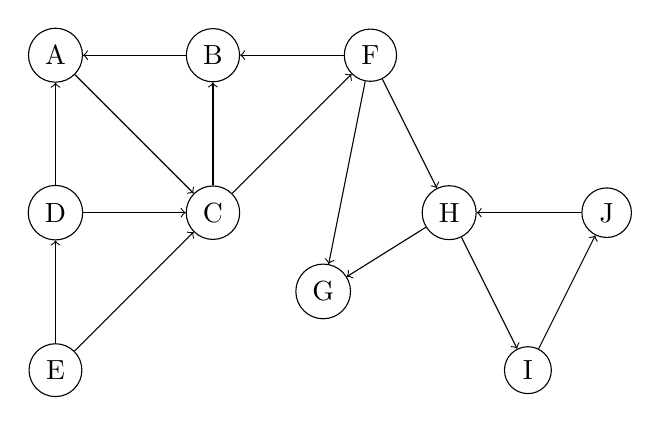
\begin{tikzpicture}[->, align=center]
\tikzstyle{v} = [circle, draw=black]
\tikzstyle{e} = [draw=black]

\node[v] (A) at (-2, 2) {A};
\node[v] (B) at (0, 2) {B};
\node[v] (C) at (0, 0) {C};
\node[v] (D) at (-2, 0) {D};
\node[v] (E) at (-2, -2) {E};
\node[v] (F) at (2, 2) {F};
\node[v] (G) at (1.4, -1) {G};
\node[v] (H) at (3, 0) {H};
\node[v] (I) at (4, -2) {I};
\node[v] (J) at (5, 0) {J};

\draw[e] (B) to (A);
\draw[e] (D) to (A);
\draw[e] (C) to (B);
\draw[e] (F) to (B);
\draw[e] (A) to (C);
\draw[e] (D) to (C);
\draw[e] (E) to (C);
\draw[e] (E) to (D);
\draw[e] (C) to (F);
\draw[e] (F) to (G);
\draw[e] (H) to (G);
\draw[e] (F) to (H);
\draw[e] (J) to (H);
\draw[e] (H) to (I);
\draw[e] (I) to (J);
\end{tikzpicture}
\end{figure}

Siden G har høyest postfixteller (20) begynner vi der. Vi ser i $ G^t $ at G ikke har noen kanter ut. Første SCC er derfor \{G\}. Når vi tar vekk G fra grafen er det H som har høyest postfixverdi (19), vi starter derfor neste dfs derfra. Vi går fra H til I og J, før vi treffer på H igjen. Vi går tilbake, men siden hverken J eller I har flere etterfølgere stopper søket, og neste SCC er derfor \{H, I, J\}. Nå er det A som har høyest postfixteller (12), så vi starter derfra. Fra A går vi til C, og til B. Da møter vi på A igjen, så vi går tilbake til C og videre til F. Vi går \emph{ikke} fra F til G eller H, siden de allerede er besøkt tidligere. Vi går derfor tilbake til C og tilbake til A. I det søke besøkte vi \{A, B, C, F\}, det blir derfor neste SCC. Til slutt starter vi i D (7), men siden D ikke har noen kanter til ubesøkte noder stopper søket med en gang. Det samme skjer i E (6). 

Alle SCCer til $ G $ er: \{ \{G\}, \{H, I, J\}, \{A, B, C, F\}, \{D\}, \{E\} \}
\end{eks}

\subsubsection{Dijkstras algoritme}
\label{dijkstra}

Dijkstras algoritme er en algoritme for å finne korteste vei fra en node til alle andre noder i en urettet graf. Algoritmen er i utgangspunktet for vektede grafer, men kan også anvendes på uvektede. Vi tenker da på en uvektet graf som en vektet graf der alle vektene er like ($ =1 $). Algoritmen er grådig siden vi alltid velger den noden med lavest avstand, og fortsetter derfra. 

\begin{teorem}Dijkstras algoritme

Vi skal finne korteste vei fra en node $ s $ til alle andre noder i en vektet, urettet graf $ G $. 
\begin{enumerate}
\item For alle noder: Sett avstanden fra startnoden $ s $ lik $ \infty $. Sett avstanden fra $ s $ til seg selv lik 0
\item Velg den naboen $ v $ til $ s $ med lavest avstand og marker den som kjent.
\item For hver nabonode $ w $ til $ v $: Dersom avstanden vi får ved å følge veien gjennom $ v $ er kortere enn den gamle avstanden, reduserer vi avstanden fra $ s $ til $ w $, og setter bakoverpekeren i $ w $ til $ v $. 
\end{enumerate}
\end{teorem}

\newpage
\noindent Vi ser på et eksempel:

\begin{eks} Finn korteste vei fra $ v1 $ til alle andre noder:
\begin{figure}[H]
\centering
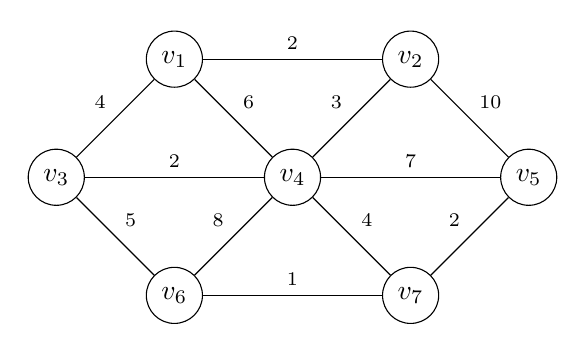
\begin{tikzpicture}[auto,node distance=2cm]
\tikzstyle{vertex} = [circle, draw=black]
\tikzstyle{edge} = [draw=black]

\node[vertex] (v1) at (-1.5,1.5) {$ v_1 $};
\node[vertex] (v2) at (1.5, 1.5) {$ v_2 $};
\node[vertex] (v3) at (-3,0) {$ v_3 $};
\node[vertex] (v4) at (0,0) {$ v_4 $};
\node[vertex] (v5) at (3,0) {$ v_5 $};
\node[vertex] (v6) at (-1.5,-1.5) {$ v_6 $};
\node[vertex] (v7) at (1.5,-1.5) {$ v_7 $};

\draw[edge] (v3) to node{\scriptsize4} (v1);
\draw[edge] (v3) to node{\scriptsize2} (v4);
\draw[edge] (v3) to node{\scriptsize5} (v6);
\draw[edge] (v1) to node{\scriptsize6} (v4);
\draw[edge] (v6) to node{\scriptsize8} (v4);
\draw[edge] (v4) to node{\scriptsize3} (v2);
\draw[edge] (v4) to node{\scriptsize4} (v7);
\draw[edge] (v4) to node{\scriptsize7} (v5);
\draw[edge] (v2) to node{\scriptsize10} (v5);
\draw[edge] (v7) to node{\scriptsize2} (v5);
\draw[edge] (v1) to node{\scriptsize2} (v2);
\draw[edge] (v6) to node{\scriptsize1} (v7);
\end{tikzpicture}
\end{figure}

\noindent Vi begynner med å sette opp en tabell over nodene:
\begin{center}
\begin{tabular}{c | c | c | l}
	 Node   & Kjent & Avstand    & Vei \\ \hline
	$ v_1 $ & T     & 0          & -   \\
	$ v_2 $ & F     & $ \infty $ & -   \\
	$ v_3 $ & F     & $ \infty $ & -   \\
	$ v_4 $ & F     & $ \infty $ & -   \\
	$ v_5 $ & F     & $ \infty $ & -   \\
	$ v_6 $ & F     & $ \infty $ & -   \\
	$ v_7 $ & F     & $ \infty $ & -
\end{tabular}
\end{center}
Vi ser på kantene ut fra $ v_1 $. Vi oppdaterer veien til $ v_2 $, $ v_3 $ og $ v_4 $:
\begin{center}
\begin{tabular}{c | c | c | l}
	 Node   & Kjent & Avstand    & Vei                    \\ \hline
	$ v_1 $ & T     & 0          & -                      \\
	$ v_2 $ & F     & $ 2 $      & $ v_1 \leftarrow v_2 $ \\
	$ v_3 $ & F     & $ 4 $      & $ v_1 \leftarrow v_3 $ \\
	$ v_4 $ & F     & $ 6 $      & $ v_1 \leftarrow v_4 $ \\
	$ v_5 $ & F     & $ \infty $ & -                      \\
	$ v_6 $ & F     & $ \infty $ & -                      \\
	$ v_7 $ & F     & $ \infty $ & -
\end{tabular}
\end{center}
Nå kommer Dijkstras grådige kriterium: Vi velger den noden som har lavest avstand til $ v_1 $ og som ikke er kjent, altså $ v_2 $ og fortsetter derfra. Fra $ v_2 $ har vi kant til $ v_4 $ og $ v_5 $. Ved å gå via $ v_2 $ får vi litt kortere avstand mellom $ v_4 $ og $ v_1 $. Vi oppdaterer tabellen:
\begin{center}
\begin{tabular}{c | c | c | l}
	 Node   & Kjent & Avstand    & Vei                                   \\ \hline
	$ v_1 $ & T     & 0          & -                                     \\
	$ v_2 $ & T     & $ 2 $      & $ v_1 \leftarrow v_2 $                \\
	$ v_3 $ & F     & $ 4 $      & $ v_1 \leftarrow v_3 $                \\
	$ v_4 $ & F     & $ 5 $      & $ v_1 \leftarrow v_2 \leftarrow v_4 $ \\
	$ v_5 $ & F     & $ 12 $     & $ v_1 \leftarrow v_2 \leftarrow v_5 $ \\
	$ v_6 $ & F     & $ \infty $ & -                                     \\
	$ v_7 $ & F     & $ \infty $ & -
\end{tabular}
\end{center}
Neste ukjente node med lavest avstand er $ v_3 $. Vi fortsetter derfra. De neste stegene ser slik ut:
\begin{center}
\begin{tabular}{c | c | c | l}
	 Node   & Kjent & Avstand    & Vei                                   \\ \hline
	$ v_1 $ & T     & 0          & -                                     \\
	$ v_2 $ & T     & $ 2 $      & $ v_1 \leftarrow v_2 $                \\
	$ v_3 $ & T     & $ 4 $      & $ v_1 \leftarrow v_3 $                \\
	$ v_4 $ & F     & $ 5 $      & $ v_1 \leftarrow v_2 \leftarrow v_4 $ \\
	$ v_5 $ & F     & $ 12 $     & $ v_1 \leftarrow v_2 \leftarrow v_5 $ \\
	$ v_6 $ & F     & $ 9 $      & $ v_1 \leftarrow v_3 \leftarrow v_6 $ \\
	$ v_7 $ & F     & $ \infty $ & -
\end{tabular}~~
\begin{tabular}{c | c | c | l}
	 Node   & Kjent & Avstand & Vei                                                  \\ \hline
	$ v_1 $ & T     & 0       & -                                                    \\
	$ v_2 $ & T     & $ 2 $   & $ v_1 \leftarrow v_2 $                               \\
	$ v_3 $ & T     & $ 4 $   & $ v_1 \leftarrow v_3 $                               \\
	$ v_4 $ & T     & $ 5 $   & $ v_1 \leftarrow v_2 \leftarrow v_4 $                \\
	$ v_5 $ & F     & $ 12 $  & $ v_1 \leftarrow v_2 \leftarrow v_5 $                \\
	$ v_6 $ & F     & $ 9 $   & $ v_1 \leftarrow v_3 \leftarrow v_6 $                \\
	$ v_7 $ & F     & $ 9 $   & $ v_1 \leftarrow v_2 \leftarrow v_4 \leftarrow v_7 $
\end{tabular}
\end{center}

\begin{center}
\begin{tabular}{c | c | c | l}
	 Node   & Kjent & Avstand & Vei                                                  \\ \hline
	$ v_1 $ & T     & 0       & -                                                    \\
	$ v_2 $ & T     & $ 2 $   & $ v_1 \leftarrow v_2 $                               \\
	$ v_3 $ & T     & $ 4 $   & $ v_1 \leftarrow v_3 $                               \\
	$ v_4 $ & T     & $ 5 $   & $ v_1 \leftarrow v_2 \leftarrow v_4 $                \\
	$ v_5 $ & F     & $ 12 $  & $ v_1 \leftarrow v_2 \leftarrow v_5 $                \\
	$ v_6 $ & T     & $ 9 $   & $ v_1 \leftarrow v_3 \leftarrow v_6 $                \\
	$ v_7 $ & F     & $ 9 $   & $ v_1 \leftarrow v_2 \leftarrow v_4 \leftarrow v_7 $
\end{tabular}
\end{center}
\begin{center}
\begin{tabular}{c | c | c | l}
	 Node   & Kjent & Avstand & Vei                                                                 \\ \hline
	$ v_1 $ & T     & 0       & -                                                                   \\
	$ v_2 $ & T     & $ 2 $   & $ v_1 \leftarrow v_2 $                                              \\
	$ v_3 $ & T     & $ 4 $   & $ v_1 \leftarrow v_3 $                                              \\
	$ v_4 $ & T     & $ 5 $   & $ v_1 \leftarrow v_2 \leftarrow v_4 $                               \\
	$ v_5 $ & F     & $ 11 $  & $ v_1 \leftarrow v_2 \leftarrow v_4 \leftarrow v_7 \leftarrow v_5 $ \\
	$ v_6 $ & T     & $ 9 $   & $ v_1 \leftarrow v_3 \leftarrow v_6 $                               \\
	$ v_7 $ & T     & $ 9 $   & $ v_1 \leftarrow v_2 \leftarrow v_4 \leftarrow v_7 $
\end{tabular}
\end{center}
\begin{center}
\begin{tabular}{c | c | c | l}
	 Node   & Kjent & Avstand & Vei                                                                 \\ \hline
	$ v_1 $ & T     & 0       & -                                                                   \\
	$ v_2 $ & T     & $ 2 $   & $ v_1 \leftarrow v_2 $                                              \\
	$ v_3 $ & T     & $ 4 $   & $ v_1 \leftarrow v_3 $                                              \\
	$ v_4 $ & T     & $ 5 $   & $ v_1 \leftarrow v_2 \leftarrow v_4 $                               \\
	$ v_5 $ & T     & $ 11 $  & $ v_1 \leftarrow v_2 \leftarrow v_4 \leftarrow v_7 \leftarrow v_5 $ \\
	$ v_6 $ & T     & $ 9 $   & $ v_1 \leftarrow v_3 \leftarrow v_6 $                               \\
	$ v_7 $ & T     & $ 9 $   & $ v_1 \leftarrow v_2 \leftarrow v_4 \leftarrow v_7 $
\end{tabular}
\end{center}
\end{eks}

\paragraph{Tidsanalyse}~\\
Hvis vi søker gjennom grafen etter den noden med lavest avstand vil det ta $ O(|V|) $ tid, og dette gjør vi $ |V| $ ganger. Total tid for å finne minste avstand er derfor $ O(|V|^2) $. I tillegg må vi oppdatere avstandene. Det er maksimalt én oppdatering for hver kant, det vil si at det tilsammen tar $ O(|E|) $. Total kjøretid for algoritmen er derfor:
\[ \text{Kjøretid} = O\left(|V|^2 + |E|\right) = O\left(|V|^2\right) \]

\subsubsection{Prims algoritme}
\label{prim}

Prims algoritme er en algoritme for å finne minimale spenntrær. Det er en grådig algoritme siden den bygger treet trinnvis ved å velge den kanten som går ut av treet med lavest vekt. 

\begin{teorem} Prims algoritme

Vi skal finne et minimalt spenntre for en graf $ G $. Velg først en startnode (rotnode). Den kan velges helt tilfeldig. Så lenge treet ikke spenner hele $ G $ legger vi til den kanten fra treet, til en ukjent node som har lavest vekt.
\end{teorem}

\noindent Vi ser på et eksempel.

\begin{eks} Finn et minimalt spenntre for grafen i figur \ref{fig:min_spenntre}.

Vi velger $ v_1 $ som rotnode (vi kunne valgt hvilken som helst annen). Den kanten med lavest vekt ut fra treet (som kun består av $ v_1 $) er kanten $ v_1-v_4 $, så vi legger den til. Videre er kanten $ v_1-v_2 $ den kanten med lavest vekt som går til en ukjent node, så vi legger til den. $ v_4-v_3 $ er neste kant vi legger til. Kanten $ v_2-v_4 $ er nå den kanten med lavest vekt som går ut fra treet, men siden $ v_2 $ og $ v_4 $ begge er inneholdt i treet er ikke den interessant. Neste kant vi legger til er $ v_4-v_7 $, deretter $ v_7-v_6 $ og $ v_7-v_5 $. Treet er nå et komplett spenntre for $ G $. 
\end{eks}

\paragraph{Tidsanalyse}~\\
Samme argument som tidsanalysen til Dijkstra. Total kjøretid: $ O\left(|V|^2\right) $


\subsubsection{Kruskals algoritme}
\label{kruskal}

Kruskals algoritme er en annen algoritme for å finne minimale spenntrær. Det er også en grådig algoritme, siden vi til enhver tid velger den kanten med lavest vekt som ikke danner en løkke.

\begin{teorem} Kruskals algoritme

Vi skal finne et minimalt spenntre for en graf $ G $. La $ F $ være en skog (en mengde av trær). Så lenge $ F $ ikke utspenner alle nodene velger vi den kanten med lavest vekt fra $ G $, og som ikke danner en løkke, og legger den til i $ F $. Når $ F $ har blitt ett sammenhengende tre og alle nodene er nådd har vi et minimalt spenntre.
\end{teorem}

\noindent Vi ser på et eksempel.

\begin{eks} Finn et minimalt spenntre for grafen i figur \ref{fig:min_spenntre}.

Vi finner kanten(e) i grafen med den minste vekten. $ v_6-v_7 $ og $ v_1-v_4 $ har begge vekt 1. Vi legger de til i spenntreet. Kantene $ v_3-v_4 $ og $ v_1-v_2 $ har begge vekt 2, og ingen av dem danner en løkke, så vi legger dem til i spenntreet. Neste kant med lavest vekt er $ v_2-v_4 $ (3), men den vil danne en løkke, så vi hopper over den. Videre ser vi at $ v_1-v_3 $ og $ v_4-v_7 $ begge har vekt 4. Kanten $ v_1-v_3 $ vil danne en løkke så den hopper vi over, men $ v_4-v_7 $ legger vi til. Neste kant med lavest vekt, og som ikke danner en løkke er $ v_5-v_7 $. Vi legger den til i spenntreet, og da er alle noder nådd, og vi har en sammenhengende graf. Vi har derfor et minimalt spenntre (se figur \ref{fig:min_spenntre}). 
\end{eks}


\paragraph{Tidsanalyse}~\\
Vi må loope gjennom alle kantene én gang, det gir tid $ O(|E|) $. Vi kan implementere algoritmen ved hjelp av en stack. Gjør vi det må vi utføre én sletting, to søk og en union. Sletting og søk tar $ O(\log_2 n) $ tid (for sletting er $ n = |E| $, for søk er $ n = |V| $), og union tar $ O(1) $ tid. For hver iterasjon har vi da:

\[ \text{Kjøretid, hver iterasjon} ~=~ O(\log_2 |E| + \log_2 |V| + 1) ~=~ O(\log_2 |V|) \]

\noindent Siste likhet har vi siden $ |V| > |E| $. Vi kan dermed sette opp total kjøretid:

\[ \text{Kjøretid, total} ~=~ O(|E| \cdot \log_2 |V|) \]


~\\
\paragraph{Prim vs Kruskal}~\\
Prim er som regel noe mer effektiv enn Kruskal, spesielt på tette grafer. Prim har likevel den svakheten at den kun fungerer på sammenhengende grafer. Kruskal anvendt på en usammenhengende graf vil gi et minimalt spenntre for hver sammenhengende del av grafen.


\subsubsection{Floyds algoritme}
\label{floyd}

Floyds algoritme er en algoritme som beregner korteste vei fra alle noder til alle andre noder. Algoritmen er et eksempel på en algoritme som benytter seg av dynamisk programmering. 

\begin{teorem} Floyds algoritme

Denne betraktningen gjentas systematisk for alle tripler i, k og j:
\begin{itemize}
\item Initielt: Avstanden fra node $ i $ til node $ j $ settes lik vekten på kanten fra $ i $ til $ j $, uendelig hvis det ikke går noen kant fra $ i $ til $ j $
\item Trinn 0: Se etter forbedringer ved å velge node 0 som mellomnode
\item Etter trinn $ k $: Avstanden mellom to noder er den korteste veien som bare bruker nodene $ 0, 1, ... , k $ som mellomnoder
\end{itemize}
\end{teorem}

\noindent Eksempel på implementasjon i Java:
\javaimport{kode/floyd.java}

\paragraph{Tidsanalyse}~\\
Vi ser fra kodeeksempelet at det er to løkker som må kjøres gjennom. En dobbel og en trippel for-løkke. Kjøretiden blir derfor:

\[ \text{Kjøretid} ~=~ O\left(n^2 + n^3\right)  ~=~ O\left(n^3\right) \]

~\\
\paragraph{Hvordan tolke input/output fra Floyds algoritme}~\\
Ved start inneholder \verb|nabo[i][j]| lengden av kanten fra $ i $ til $ j $, \verb|nabo[i][j] = |$ \infty $ hvis det ikke er noen kant. Algoritmen lar \verb|nabo| være uendret, og legger resultatene i \verb|avstand| og \verb|vei|. \verb|avstand[i][j]| er lengden av korteste vei fra $ i $ til $ j $. Når vi oppdager at den korteste veien fra $ i $ til $ j $ går gjennom $ k $ setter vi \verb|vei[i][j] = k|. \verb|vei| sier derfor om den korteste veien. Vi finner korteste vei slik:
\begin{itemize}
\item \verb|k1 = vei[i][j]| er den største verdien av $ k $ slik at $ k $ ligger på den korteste veien fra $ i $ til $ j $
\item \verb|k2 = vei[i][k1]| er den største verdien av $ k $ slik at $ k $ ligger på den korteste veien fra $ i $ til $ k_1 $
\\ $ \vdots $
\item Når \verb|vei[i][km] = -1| er $ (i, k_m) $ den første kanten i korteste vei fra $ i $ til $ j $
\end{itemize}
Dermed er korteste vei fra $ i $ til $ j $ slik: $ i \rightarrow k_m \rightarrow k_{m-1} \rightarrow ... \rightarrow k_2 \rightarrow k_1 \rightarrow j $. 				% ferdig, mangler indexer
\newpage
\section{Andre datastrukturer}
\subsection{Heap (prioritetskø)}\label{heap}
En heap (også kalt prioritetskø) er en type binært tre med noen spesielle struktur- og ordningskrav. Vi har to typer heap: min- og maksheap. Vi vil beskrive minheap i dette kapitlet, men maksheap fremgår helt analogt.

\begin{definition} En minheap er et binært tre der følgende krav er oppfylt:  \label{def:heap}
\begin{enumerate}
\item Treet er komplett (høyden til treet er $ \lceil\log_2 n\rceil $)
\item En node har alltid (sorterings)verdi mindre enn, eller lik sine barn. 
\end{enumerate}
\end{definition}

En maksheap defineres nesten likt, eneste forskjell er at pt. 2 i definisjonen blir ``En node alltid er større enn, eller lik sine barn.''

Hver node i en heap inneholder to ting: et element, og en verdi vi sorterer etter. I motsetning til i et binært søketre der vi sorterer på elementet selv, vil vi med en heap tilordne en sorteringsverdi til hvert element som ikke trenger å ha noe med elementet å gjøre. 

~\\
\begin{figure}[H]
\centering
\caption{En (min)heap. For oversiktens skyld er kun sorteringsverdiene tatt med.}
\label{fig:heap}
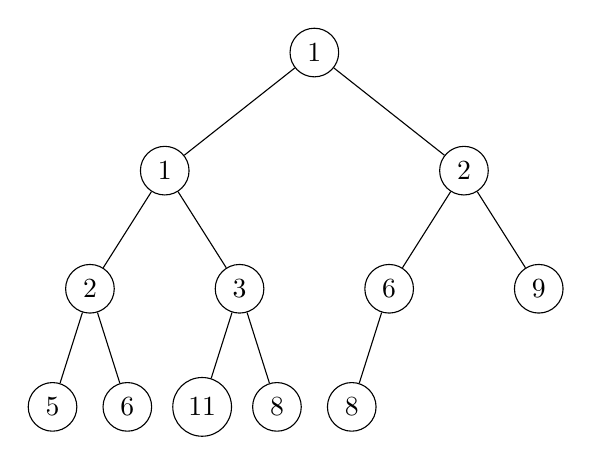
\begin{tikzpicture}[level distance=1.5cm,
  level 1/.style={sibling distance=3.8cm},
  level 2/.style={sibling distance=1.9cm},
  level 3/.style={sibling distance=0.95cm},
every node/.style = {shape=circle, draw, align=center}]

\node{1}
	child {node {1}
		child {node {2}
			child {node {5}}
			child {node {6}}
		}
		child {node {3}
			child {node {11}}
			child {node {8}}
		}
	}
	child {node {2}
		child {node {6}
			child {node {8}}
			child [missing] {}
		}
		child {node {9}}
	};
\end{tikzpicture}
\end{figure}

\paragraph{Innsetting}~\\
Når vi skal sette inn et element i en heap setter vi den på første ledige plassen. Deretter sammenligner vi nodens verdi med forelderens verdi. Hvis forelderen har større verdi enn noden vi setter inn bytter vi plass\footnote{Foreleser og lærebok kaller denne prosessen \say{percolate up}}. Så sammenligner vi med den nye forelderen, bytter plass om nødvendig, og fortsetter slik til enten forelderen er mindre enn noden, eller at noden er rot. 

\paragraph{Fjerning (deleteMin)}~\\
I en heap er vi egentlig bare interessert i å ta ut det minste elementet fra en heap (hvorfor blir diskutert i avsnittet om anvendelser). På grunn av krav 2 i definisjonen vet vi at rota er det minste elementet i heapen. Derfor fjerner vi rota. For å skaffe en ny rot tar vi det siste elementet i heapen og setter som rot. Deretter sammenligner vi verdien av den nye rota med verdien av barna. Hvis et (eller begge) av barna har mindre verdi enn den nye rota bytter rota plass med \textbf{det minste} barnet\footnote{\say{percolate down}}. Vi fortsetter slik til ordningskravet er oppfylt (noden har mindre verdi enn barna). 

\paragraph{Implementasjon}~\\
Vi kan implementere en heap som et tre (dvs, lage nodeobjekter med pekere til barn etc), men som oftest implementerer vi en heap ved hjelp av en array. Vi lar rota være på index 1. På grunn av kompletthetskravet kan vi legge nodene radvis bak rota. Vi finner da barna til en node på index $ i $ ved å til index $ 2i $ (venstre barn) og $ 2i+1 $ (høyre barn), og forelder ved å gå til index $ \lfloor i/2 \rfloor $. Når vi implementerer en heap som en array kan vi risikere å gå tom for plass i arrayen. Da må vi lage en ny array, og flytte over alle elementene til den nye arrayen. Vanligvis legger vi til en og en rad i slengen (eventuelt to og to, tre og tre, etc..). Å gjøre dette tar åpenbart $ O(n) $ tid, men vi må gjøre det sjeldnere og sjeldnere jo større heapen blir. 

\begin{figure}[H]
\centering
\caption{Heapen i fig \ref{fig:heap} representert som array}
\begin{tabular}{r||c|c|c|c|c|c|c|c|c|c|c|c|c|c|c|c}
	~~index &  0   & 1 & 2 & 3 & 4 & 5 & 6 & 7 & 8 & 9 & 10 & 11 & 12 &  13  &  14  &  15  \\ \hline
	~~verdi & null & 1 & 1 & 2 & 2 & 3 & 6 & 9 & 5 & 6 & 11 & 8  & 8  & null & null & null 
\end{tabular}
\end{figure}

I Java har vi en ferdig heap: \mono{java.util.PriorityQueue<E>}. Java krever at \mono{E} er sammenlignbar med seg selv (\mono{E} implementerer \mono{comparable<E>}) og vil bruke den sammenligningen som grunnlag for sortering. Javas heap er implementert som array. 

\paragraph{Tidsanalyse}~\\
Vi ser på kjøretiden til de to omtalte operajonene:
\begin{theorem} Kjøretid for heapoperasjoner \label{teo:heapop}
\begin{enumerate}[i]
\item Innsetting i en heap tar $ O(\log_2 n) $ tid
\item Fjerne minste element tar $ O(\log_2 n) $ tid
\end{enumerate}
\end{theorem}
Beviset følger av strukturkravet i definisjon \ref{def:heap}:
\begin{proof} Teorem \ref{teo:heapop}, del i:

Når vi setter inn et element i en heap må vi først sette elementet på slutten av heapen. Siden vi vet hvor siste element er vil dette ta $ O(1) $ tid. Deretter må vi justere plassen til elementet ved å la elementet sive oppover. Siden treet er komplett vil høyden på treet være $ \lceil\log_2 n\rceil $, og vi kan maksimalt foreta $ \lceil\log_2 n\rceil - 1 $ byttinger. Total tid blir derfor være $ O(\log_2 n) $
\end{proof}
Argumentet for teo. \ref{teo:heapop}, del ii er helt analogt. 


\paragraph{Anvendelser}~\\
I dette kurset ser vi på to anvendelser av en heap: Prioritetskø og sortering. Når vi bruker en (min)heap som en prioritetskø lar vi viktige jobber ha lav verdi, og mindre viktige jobber ha høy verdi. Når vi setter jobbene våre inn i en heap og tar dem ut vil de viktigste jobbene komme først. Fordelen med dette mot å bare sortere lista med jobber er at vi dynamisk kan legge til flere jobber underveis. 

Vi kan også sortere en liste med elementer ved hjelp av en heap. Se \ref{heapsort}.



\subsubsection{Venstreorientert (leftist) heap}
En venstreorientert heap er en en heap med et annet strukturkrav enn vanlig heap. Motivasjonen bak venstreorienterte heaper er at å flette (merge) to heaper av samme størrelse tar $ O(n) $ tid, vi ønsker å forbedre det. Før vi kan definere en venstreorientert heap må vi definere \say{null path length} (herfra: npl). Npl til en node $ n $ er lengden av den korteste veien fra $ n $ til en etterkommer uten to barn ($ 0 $ hvis $ n $ har $ <2 $ barn). 

\begin{definition} En venstreorientert heap er et binært tre der følgende krav er oppfylt:
\begin{enumerate}
\item For hver node $ n $ i treet er $ \text{npl}(l) \geq \text{npl}(r) $, der $ l $ er venstre og $ r $ er høyre barn til $ n $.
\item En node har alltid (sorterings)verdi mindre enn, eller lik sine barn. 
\end{enumerate}
\end{definition}

\begin{figure}[H]
\centering
\caption{Et tre med $ \text{npl}(n) $ skrevet inn}
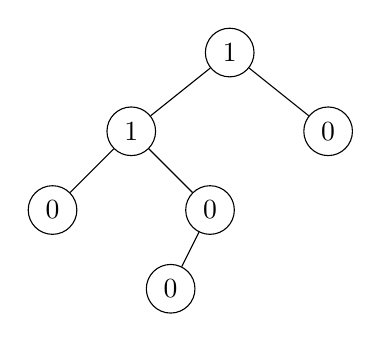
\begin{tikzpicture}[level distance=1cm,
  level 1/.style={sibling distance=2.5cm},
  level 2/.style={sibling distance=2cm},
  level 3/.style={sibling distance=1cm},
every node/.style = {shape=circle, draw, align=center}]

\node{1}
child {
	node {1}
	child {
		node {0}
	}
	child {
		node {0}		
		child {
			node {0}
		}
		child[missing]
	}
}
child {
	node {0}
};
\end{tikzpicture}
\end{figure}

\noindent \textbf{Merk:} En venstreorientert heap forsøker å være ute av balanse (for å gjøre fletting enklere).

\paragraph{Operasjoner}~\\
Hovedoperasjonen på venstreorienterte heaper er \textbf{fletting} (engelsk: merging). Vi kan implementere fletting rekursivt: Når vi skal flette to heaper $ H_1 $ og $ H_2 $ sammenligner vi først røttene. La $ H_1 $ være heapen med minst rot. La så den høyre subheapen til $ H_1 $ være heapen som fremstår ved å flette høyre subheap i $ H_1 $ med hele $ H_2 $. Vi fortsetter slik til problemet er trivielt. Gjennomgående kan vi bytte om høyre og venstre subheap for å bevare strukturkravet (def. pt. 1).

For å \textbf{sette inn} en node i en venstreorientert heap kan vi flette en heap bestående av den ene noden vi vil sette inn, med hele heapen vi vil sette noden inn i.

For å \textbf{fjerne} minste node kan vi ta vekk rota (som vi vet er minst fra def. pt. 2), og flette venstre og høyre subheap.





\subsection{Hashmap (hashtabell)} \label{hashmap}
Sett at vi har en liste med $ n $ elementer. Vi skal søke etter et element $ x $. Hvis vi har implementer lista vår som en array eller lenket liste vil dette ta $ O(n) $ tid. Det vil også operasjoner som sletting, og å sette inn på første ledige plass. Vi ønsker å finne en datastruktur som er bedre på disse tingene. 

Den grunnleggende idéen bak hashtabeller er å la verdien til elementet vi skal sette inn bestemme indexen. Vi bruker en hashfunksjon $ f:\mathbb{N}\rightarrow\mathbb{N} $ på elementet vårt $ x $, og lar $ f(x) $ betegne indexen til elementet i en array. 

\begin{itemize}
\item Når vi oppretter en hashtabell lager vi en ny array som er $ tableSize $ lang. Størrelsen på arrayen er et primtall. 
\item Når vi skal sette inn et element $ x $ i en hashtabell regner vi ut $ f(x) $ og setter $ x $ inn i arrayen på plass $ f(x) $
\item Når vi skal søke etter et element $ x $ i hashtabellen regner vi ut $ f(x) $ og slår opp på den plassen i arrayen. Hvis elementet er der har vi funnet det. Hvis elementet ikke er der må vi muligens sjekke noen andre steder. Hvor vi må lete videre avhenger av hvordan vi håndterer like hashresultater. 
\item Når vi skal fjerne et element $ x $ i en hashtabell søker vi opp elementet i tabellen, og sletter det. 
\end{itemize}

\noindent Et eksempel på en hashfunksjon kan være $ f(x) = x \mod tableSize $

~\\
\subsubsection{Håndtering av like hashresultater}
Hashfunksjoner trenger ikke å være injektive. Det vil si at vi fort kan få $ f(x) = f(y) $ selv om $ x \neq y $. Hvis vi skal sette inn $ y $ i en hashtabell, men plassen med index $ f(y) $ allerede er okkupert av $ x $ må vi finne en ny plass til $ y $. Det kan gjøres på flere måter, vi deler opp i to hovedgrupper: Seperate chaining og probing. 


\paragraph{Seperate chaining}~\\
En mulig løsning på problemet med like hashresultater er å la arrayen vår være en array av lenkede lister. Vi kan dermed ha flere elementer i hver index. Når vi skal sette inn $ x $, regner vi ut $ f(x) $, og setter y bakerst i lista på den plassen. Dermed har det ingenting å si om det eksisterer elementer på indexen eller ikke. 

Problemet med seperate chaining er at vi må tråkke oss gjennom en lenket liste etter at vi har funnet hashresultatet. Dette tar lineær tid (men dog med (forhåpentligvis) færre elementer enn $ n $)


\paragraph{Lineær probing}~\\
En annen mulig løsning på problemet er å gå til plassen bak $ f(x) $, og hvis den er opptatt går vi til indexen bak det igjen. Skulle vi komme til enden av arrayen begynner vi fra toppen igjen. Generelt for probing har vi at plassen vi setter elementet inn på er gitt ved
\[ index = (f(x) + g(k)) \mod{tableSize} \]
der $ f $ er hashfunksjonen, $ g $ er i dette tilfellet $ g(k) = k $, $ k $ er antall skritt vi har tatt fra den opprinnelige indexen (antall ganger vi har støtt på et element) og $ tableSize $ er antall plasser i tabellen. Igjen får vi det problemet at vi i praksis må søke igjennom en liste etter å ha funnet hashresultatet. 

\paragraph{Kvadratisk probing}~\\
Kvadratisk probing ligner veldig på lineær probing, med den forskjellen at $ g(k) = k^2 $. Vi går altså til den plassen som ligger $ 1, 4, 9, ... $ plasser bak $ f(x) $

\paragraph{Dobbel hashing}~\\
Med dobbel hashing har vi en ekstra hashfunksjon $ f_2(x) $ som vi regner ut hvis vi skulle støte på problemer. Vi får da at $ g(k) = k f_2(x) $. Et eksempel på en funksjon $ f_2 $ kan være $ f_2(x) = R-(x \mod R) $ der $ R $ er det største primtallet som er mindre enn $ tableSize $. 

~\\
\subsubsection{Rehashing}
Hvis hashtabellen begynner å bli full kan det lønne seg å rehashe. Det betyr ganske greit å lage en ny tabell med større $ tableSize $ og flytte alle elementet over. Når vi rehasher lager vi som regel en tabell som er ca dobbelt så stor (men fortsatt primtall). Siden $ f $ ofte avhenger av $ tableSize $ må vi regne ut alle hashverdiene på nytt. Rehashing er derfor en ganske dyr affære, så vi gjør det veldig sjeldent, men hvis tabellen begynner å bli for full kan vi tjene ganske mye tid i lengden. 

~\\
\subsubsection{Gode hashfunksjoner}
Vi står helt fritt til å velge hashfunksjoner selv. Gode hashfunksjoner er raske å regne ut, kan gi alle mulige verdier fra $ 0 $ til $ tableSize - 1 $, og har en god fordeling (spredning). utover tabellindexene. 

Ofte bruker vi strenger som nøkler. Vi må derfor ha en måte å regne ut et tall av en tekststreng på. Det kan gjøres på mange måter, her er et par eksempler:
\begin{itemize}
\item Summer verdiene til hvert tegn:
\[ f(x) = \left( \sum_{i=0}^{keyLength-1} = \text{charVal}(key_i) \right) \mod{tableSize} \]
der $ \text{charVal} $ er en funksjon som tilordner en numerisk verdi til hver bokstav, feks ascii/unicode-verdien til tegnet. $ key_i $ betegner det $ i $-te tegnet i $ key $. Denne funksjonen er rask og enkel å implementere, men vil gi dårlig spredning for store tabeller. 
\item En vektet sum av de tre første tegnene:
\[ f(x) = \left( c_1\,\text{charVal}(key_1) + c_2\,\text{charVal}(key_2) + c_3\,\text{charVal}(key_3)\right)  \mod{tableSize} \]
der $ c $-ene er konstanter vi velger. Denne er rask å enkel å beregne, og gir en grei fordeling for tilfeldige strenger, problemet er at naturlig språk ikke er tilfeldig.
\end{itemize}


\subsubsection{Tidsanalyse}
Det er åpenbart at best case tid for innsetting, søking og fjerning i hashtabeller er $ O(1) $. Det oppstår når vi kommer rett til elementet/tom index på første forsøk. Worst case er når vi får kollisjoner på hvert eneste treff, og vi i praksis har en liste. Da vil alle operasjoner på tabellen være $ O(n) $. 

Vi ser at en tabell starter som $ O(1) $, og beveger seg mot $ O(n) $ når den blir fullere. Det er derfor vi ofte velger å rehashe når tabellen blir for full. Selv om rehashing har $ O(n) $ tid, er det en operasjon vi gjør én gang. Det vil forbedre kjøretiden på alle andre operasjoner drastisk, siden det er mindre sannsynlighet for å få kollisjoner i en tabell med mindre tetthet. Som regel prøver vi å holde andelen av tabellen som er opptatt (kalt \say{load factor}, ofte forkortet $ LF $) under en gitt grense. Java sin innebygde \mono{HashMap<K,V>} tvinger $ LF < 0.75 $.





\subsection{Kø/stack} \label{ko_stack}
Kø og stack er to forskjellige typer lister. Felles for dem er at vi kun opererer med én \mono{insert()}- og én \mono{remove()}-metode. Forskjellen er hvilket element vi vil hente ut når vi kaller \mono{remove()}-metoden. Innsetting og fjerning i både kø og stack tar $ O(1) $ tid, siden vi på forhånd vet hvor elementet skal fjernes fra/legges til. 


\subsubsection{Kø (FIFO)}
En kø er en liste der første element inn er det første som kommer ut, derav navnet. Vi kaller også slike lister for FIFO-lister (First In, First Out). Elementene som settes inn stilles bakerst i køen, og når vi henter ut et element starter vi foran. 


\subsubsection{Stack (LIFO)}
En stack (norsk: stabel) er en liste der siste element som settes inn er det første som kommer ut. Slike lister kalles også LIFO-lister (Last In, First Out). Elementene som settes inn legges på toppen av stabelen, og når vi skal hente ut et element henter vi det øverste elementet. 

Konvensjonelt kalles insert-metoden i en stack \mono{push()}, og remove-funksjonen \mono{pop()}


\newpage
\section{\color{red}Tekstalgoritmer}
	Generelt problem: Vi er interesserte i å finne ut om en streng er en substreng av en annen streng. Vi kaller substringen for en nål $i$, av lengde $m$, og stringen for en høystakk $h$, av lengde $n$.

	\subsection{Brute force}
		Brute force-metoden er som navnet tilsier ikke spesielt gjennomtenkt: Til å begynne med sjekker vi hver karakter i høystakken mot den første i nåla. Hvis vi har likhet sjekker vi det neste tegnet i høystakken mot det neste i nåla. Vi fortsetter slik til vi enten finner hele nåla i høystakken eller til vi har ulikhet, og i så fall fortsetter vi med å sjekke det neste tegnet i høystakken mot det første i nåla.

	\subsubsection{Analyse}
		Worst case så får vi mismatch $(n-m)$ ganger og suksess $(n-m)+1$ ganger, Totale sammenligninger er $((n-m)+1\times m)$ som gir kjøretid $O(n^2)$.

	\subsection{\color{red}Boyer-Moore}
		Dette er en rask substringalgoritme. Med Boyer-Moore preprosserer vi nåla før vi begynner å søke. Vi regner ut hvor mange hopp vi kan gjøre for hvert enkelt tegn i nåla ved mismatch. Dette er bad character shift. Good character shift også... Algoritmen starter med å sjekke halen på nåla og ved eventuell match beveger seg mot venstre. Fortsetter så enten til hele nåla er matchet eller til mismatch, hvor vi i så fall beveger oss \verb|badShift[i]| bortover.

	\subsubsection{\color{red}Bad character shift}
		Vi beregner avstand til neste gang nål er på linje med høystakk\ref{huffman}.
	\subsubsection{\color{red}Good suffix shift}
		Vi bruker antall match før mismatch for å finne skip-avstand.

	\subsection{\color{red}Huffmankoding}\label{huffman}
		\begin{enumerate}
			\item Lager frekvenstabell for alle tegn som forekommer i teksten.
			\item Betrakt hvert tegn som en node og legg alle noder i en prioritetskø (heap). Se \ref{heap}.
			\item Mens P har mer enn ett element:
				%\begin{itemize}
					
				%\end{itemize}
		\end{enumerate}
\newpage
\section{\color{red}Sortering}
\subsection{Formaliteter}
\label{sort_form}
Før vi kan begynne å se på noen spesielle sorteringsalgoritmer må vi formalisere hva vi mener med sortering. Vi definerer sortering slik:

\begin{definisjon}
Anta at $ \{a_i\}_{i=0}^n $ er en liste av sammenlignbare elementer. Vi sier at $ \{a'_i\}_{i=0}^n $ er den tilhørende sorterte lista hvis følgende kriterier er oppfylt:
\begin{enumerate}[i]
\item $ a'_i \leq a'_{i+1} $ for alle $ i = 0, 1, ..., n-1 $
\item Alle elementene i $ \{a\} $ er med i $ \{a'\} $
\end{enumerate}
\end{definisjon}

Det andre kriteriet kan virke litt snodig, men uten det ville sortering vært veldig enkelt. Vi kunne i så fall bare generert en ny liste med elementer i sortert rekkefølge, og det første kriteriet ville vært oppfylt. Vi trenger derfor bevaringskriteriet. 

Med ``sammenlignbare'' mener vi at det finnes en måte å entydig bestemme om et element er større enn, mindre enn eller lik et annet element. Hvis vi skal sortere tall er jobben enkel: vi sammenligner numerisk verdi. Hvis vi skal sammenligne to tekststrenger er det ikke like opplagt hvordan vi skal gjøre det. Skal vi sortere alfabetisk? Etter lengde på ordet? I et sånt tilfelle er det opp til oss å velge et fornuftig sammenligningskriterie. Det er vilkårlig hvordan vi sammenligner to elementer, så lenge vi gjør det likt gjennom hele sorteringen. 


\subsection{\color{red}Noen algoritmer}
Vi skal nå se på noen konkrete sorteringsalgoritmer. Gjennomgående i alle eksempler vil vi sortere tall etter tallverdi, men som diskutert i \ref{sort_form} vil vi enkelt kunne tilpasse algoritmene til å sortere på andre kriterier. 


\subsubsection{\color{red}Boblesortering}
\label{bubble}
\textbf{Boblesortering} (\textbf{bubble/(sinking) sort})  er en veldig ineffektiv sorteringsalgoritme, og brukes derfor lite i den virkelige verden. 
Idéen bak er derimot forholdsvis enkel:
Vi parvis sammenligner naboer i lista, og bytter om plassene deres dersom de står på feil plass.

\paragraph*{Wikipedias utgave}
Wikipedias versjon av boblesortering er forskjellig fra den som er gjennomgått i forelesning.
Her flytter vi oss hele tiden oppover i lista, og begynner på nytt når vi har kommet til slutten.
Dette gjentas helt til lista er ferdig sortert.

\begin{eks} Sortering av (5 1 2 5 8) \newline
  \textbf{Første gjennomgang}
  \begin{align*}
    (\mathbf{5}~ \mathbf{1}~ 2~ 5~ 8) \rightarrow (\mathbf{1}\, \mathbf{5} ~ 2 ~ 5 ~ 8) &\quad \text{Bytter, siden 5 > 1} \\
    (1~ \mathbf{5}~ \mathbf{4}~ 2~ 8) \rightarrow (1 ~ \mathbf{4} ~ \mathbf{5} ~ 2 ~ 8) &\quad \text{Bytter, siden 5 > 4} \\
    (1~ 4~ \mathbf{5}~ \mathbf{2}~ 8) \rightarrow (1~ 4~ \mathbf{2}~ \mathbf{5}~ 8)     &\quad \text{Bytter, siden 5 > 2} \\
    (1~ 4~ 2~ \mathbf{5}~ \mathbf{8}) \rightarrow (1~ 4~ 2~ \mathbf{5}~ \mathbf{8})     &\quad \text{Bytter ikke, siden 5 < 8}
  \end{align*}
  Deretter går vil tilbake til start og gjentar prosessen, helt til vi har gått gjennom lista uten at noen elementer har byttet plass.
  I dette tilfellet kreves tre gjennomganger.
\end{eks}

\javaimport{kode/bubbleSort.java}

\paragraph*{Utgaven presentert i forelesning}
I forelesningen ble en noe alternativ utgave av boblesortering presentert, og det kan være lurt å forholde seg til denne, siden det er denne som er pensum.
Denne utgaven ligner veldig på innstikksortering, fordi den ``bobler'' et element som står på feil plass nedover i lista helt til den står på riktig plass.

\javaimport{kode/optBubbleSort.java}




\subsubsection{\color{red}Innstikksortering}\label{insertion}
\subsubsection{\color{red}Tresortering}
\subsubsection{\color{red}Quicksort}
\label{quick}
\subsubsection{\color{red}Radix}

\subsection{\color{red}Parallell Sortering}
			% påbegynt
\newpage
\section{Bevisføring}
\subsection{Noen bevisteknikker}
\paragraph{Bevis ved selvmotsigelse}
Teknikken går ut på å gjøre noen antagelser, og vise til at det fører til en motsigelse. Da må noen av antagelsene være gale, og hvis vi kun har to muligheter (for eksempel rett/galt) kan vi konkludere med at det andre alternativet må være rett. Eksempel på et slik bevis er beviset for haltingproblemet (\ref{haltingProof})

\paragraph{Induksjon}
Bevis ved induksjon går ut på å anta at påstanden holder for alle mulige tall $ k $ opp til $ n $, og vise at det også medfører at det også holder for $ k = n+1 $. Dermed har man vist at hvis det også holder for $ n+1 $ vil det holde for $ n+2 $, også videre. Det siste man må gjøre er å \say{starte} induksjonen, med for eksempel å vise at påstanden holder for $ k=1 $ (da vil den også holde for $ k=2, 3, ... $)

\paragraph{Bevis ved moteksempel}
Skal man vise at en påstand er falsk, kan man ganske enkelt finne et eksempel som viser at den opprinnelige påstanden er falsk. Påstår jeg at alle hester er hvite, kan du motbevise den påstanden ved å vise meg en hest som er svart.



\subsection{Reduksjon}
Anta at vi har et problem $ A $, og vi lurer på om problemet er løselig eller ikke. $ A $ kan være latterlig komplekst og vanskelig å forstå, men kanskje vi kan uttrykke det på en annen måte? Hvis vi kan vise at hvis $ A $ er løselig er også $ B $ løselig, og hvis $ B $ er løselig er også $ C $ løselig. Slik kan vi fortsette til vi kommer til noe kjent, for eksempel haltingproblemet (\ref{haltingProof}). For matematikere:
\[ \text{$ A $ er løselig} \Rightarrow \text{$ B $ er løselig} \Rightarrow ... \Rightarrow \text{haltingproblemet er løselig} \]
Hvis vi kan vise en slik rekke av implikasjonspiler har vi \emph{redusert} $ A $ til haltingproblemet, og dermed vet vi at $ A $ er uløselig.  

\subsection{Noen beviser}
\subsubsection{Haltingproblemet}
Kan en Turingmaskin avgjøre om en annen Turingmaskin noen sinne vil stoppe, eller om den vil gå i evig loop, om den ser på inputen til maskinen? Som nevnt i \ref{språk} kan vi definere en språk som mengden av input som vil få en maskin til å stoppe:\index{haltingproblemet}
\[ L = \{i : M \text{ stopper på input } i \} \]
Det kan vises at en Turingmaskin som løser dette problemet \emph{ikke} kan eksistere. Det kan vises på flere måter, Alan Turing beviste det slik:

\label{haltingProof}
Vi skal bevise at haltingproblemet er uløselig, og vi skal gjøre det ved selvmotsigelse. 

Anta at vi har en Turingmaskin $ M $ som bestemmer om en annen Turingmaskin $ H $ vil stoppe, gitt input $ i $. Vi kan da bygge en annen Turingmaskin $ M' $ rundt denne som tar de samme parametrene ($ H $ og $ i $) som input, og gir resultat hvis $ M $ gir false (Altså at $ H $ ikke vil stoppe, gitt input $ i $), og går i en evig loop hvis $ M $ gir true (at $ H $ vil stoppe, gitt $ i $). 

Hva vil skje hvis vi bruker denne Turingmaskinen på seg selv? Hvis $ M $ sier at $ M' $ vil stoppe vil $ M' $ gå i en evig loop, og følgelig vil ikke $ M' $ stoppe. Hvis $ M $ sier at $ M' $ ikke vil stoppe vil $ M' $ gi et resultat, og så stoppe. Uansett får vi en motsigelse, og derfor kan ikke Turingmaskinen $ M $ eksistere. $ \hfill\qed $ \\

\noindent Beviset er analogt med Cantors diagonaliseringsargument. \color{red} kanskje du skal forklare hvorfor?\color{black}

\subsubsection{Cantors diagnoaliseringsargument}
Vi skal vise at størrelsen av $ \mathbb{R} $ er større enn $ \mathbb{N} $, altså at det er flere reelle tall enn naturlige tall. Dette er et eksempel på bevis ved selvmotsigelse. Vi skal anta at vi kan vise at $ \mathbb{R} $ og $ \mathbb{N} $ er like store, og så vise at det fører til en motsigelse.

Vi kan begynne med noe som kanskje går litt mot intuisjonen. Det er nemlig like mange rasjonelle tall som naturlige tall. For å vise dette må vi vise at vi har en 1-1-korrespondanse mellom naturlige tall og rasjonale tall. Vi starter med å liste opp \say{alle} de naturlige og rasjonale tall. Vi setter rasjonale tall inn i en tabell:

\[ \mathbb{N} = 1, 2, 3 ... \quad\quad \mathbb{Q} = \begin{tabular}{c | c c c c}
  & 1 & 2 & 3 & ... \\
  \hline
1 & $ ^1/_1 $ & $ ^2/_1 $ & $ ^3/_1 $ & ... \\
2 & $ ^1/_2 $ & $ ^2/_2 $ & $ ^3/_2 $ & ... \\
3 & $ ^1/_3 $ & $ ^2/_3 $ & $ ^3/_3 $ & ... \\
\vdots & \vdots & \vdots & \vdots & $ \ddots $
\end{tabular} \]

Sånn rent intuitivt kan det se ut som at det er mange flere rasjonale tall enn naturlige tall, men hvis vi går på skrå i tabellen over $ \mathbb{Q} $ kan vi knytte hvert rasjonalt tall til ett naturlig tall, og hvert naturlige tall til ett rasjonalt tall:

\[ 1: \frac{1}{1} \quad\quad 2: \frac{2}{1} \quad\quad 3: \frac{1}{2} \quad\quad 4: \frac{3}{1} \quad ... \]

Vi har dermed vist at vi kan skape en 1-1-korrespondanse mellom $ \mathbb{N} $ og $ \mathbb{Q} $, og dermed er de like store. 

Vi skal nå se på $ \mathbb{N} $ og $ \mathbb{R} $, altså de reelle tallene. Vi ønsker å prøve å skape en lignende 1-1-kobling som vi gjorde for de rasjonale tallene. $ \mathbb{R} $ er ikke tellbart uendelig, derfor kan vi ikke liste opp alle tallene i $ \mathbb{R} $ på samme måte som før med en smart tabell (dette er forøvrig grunnen til at $ \mathbb{R} $ er større enn $ \mathbb{N} $, vi skal nå vise \emph{hvorfor}). En ting vi kan gjøre er å liste opp naturlige tall på en side, og tilfeldige og unike reelle tall på den andre. Det har seg faktisk slik at det er flere reelle tall mellom 0 og 1 enn det er naturlige tall tilsammen, det holder å liste opp tilfeldige reelle tall mellom 0 og 1. Vi får da en slik tabell:

\begin{center}
\begin{tabular}{c | c}
$ \mathbb{N} $ & $ \mathbb{R} $ \\
\hline
1 & 0.182947... \\
2 & 0.294817... \\
3 & 0.132849... \\
\vdots & \vdots
\end{tabular}
\end{center}

Vi kan tenke oss at hvis vi fortsetter slik i all evighet vil vi til slutt ende opp med en 1-1-korrespondanse mellom $ \mathbb{R} $ og $ \mathbb{N} $. Vi vil jo aldri gå tom for naturlige eller reelle tall å ta av. Det viser seg likevel å være feil, og det er her Cantors diagonaliseringsargument kommer inn:

Vi kan nemlig lage et nytt reellt tall som ikke eksisterer i denne tabellen. Hvis vi tar første siffer fra første tall og legger til 1, andre siffer fra andre tall og legger til 1, også videre. Generelt tar vi det $ i $-te sifferet og legger til 1. Hvis tallet er 9 kan vi gå til 0\footnote{Formelt kan vi bruke klokkeaddisjon (moduloaddisjon): $ (9 + 1) \mod{10}  = 0 $}. Gjør vi det for denne tabellen får vi:

\[ 0.203...  \]

Siden dette tallet er ulikt tall nummer $ i $ i tabellen på $ i $-te siffer vet vi at det ikke er inneholdt i tabellen, og vi har dermed vist at det ikke kan lages en 1-1 korrespondanse mellom $ \mathbb{R} $ og $ \mathbb{N} $. Følgelig er $ \mathbb{R} $ større enn $ \mathbb{N} \hfill\qed$ 

\subsubsection{Antall noder i et binært tre}
Vi skal vise at antall noder $ n $ i et binært tre er begrenset slik:
\begin{equation*}
n \leq 2^{h} - 1
\end{equation*}
Vi skal vise dette ved induksjon.

Vi starter med å vise at formelen gjelder for et tre med høyde $ h=1 $:
\[ n = 2^1 - 1 = 1 \]
som åpenbart stemmer siden et tre med høyde 1 har kun 1 node, nemlig rota.

Vi antar at formelen gjelder for alle $ h $ opp til $ n $, og skal vise at det impliserer at den også gjelder for $ n+1 $. Vi har et tre $ T_1 $ med høyde $ n $:
\begin{center}
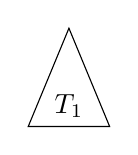
\begin{tikzpicture}[sibling distance=8em]
\node[isosceles triangle, draw=black, align=center, minimum height=0.5cm, minimum width=1cm, shape border rotate=90, anchor=north]{$ T_1 $};
\end{tikzpicture}
\end{center}
Vi antar at formelen stemmer, og dermed at antall noder i $ T_1 $ maksimalt er $ 2^n - 1 $. Vi skal nå øke høyden til $ n+1 $. Vi lager en ny rot, med to fulle subtrær som barn:
\begin{center}
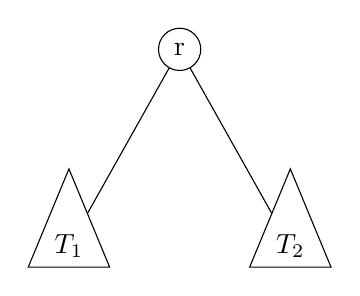
\begin{tikzpicture}[sibling distance=8em]
\node[shape=circle, draw, align=center]{r} 
	child {node[isosceles triangle, draw=black, align=center, minimum height=0.5cm, minimum width=1cm, shape border rotate=90, anchor=north]{$ T_1 $}}
	child {node[isosceles triangle, draw=black, align=center, minimum height=0.5cm, minimum width=1cm, shape border rotate=90, anchor=north]{$ T_2 $}};
\end{tikzpicture}
\end{center}
Fra formelen har vi at $ T_1 $ og $ T_2 $ maksimalt har $ 2^n-1 $ noder hver. Legger vi sammen antall noder i treet nå får vi:
\[ n ~=~ \text{noder i } T_1 + \text{noder i } T_2 + 1 ~\leq~ 2(2^n -1) + 1 ~=~ 2^{n+1} - 1 \]

Oppsummering: Vi har vist at hvis formelen gjelder for $ h=n $ gjelder den også for $ h=n+1 $, vi har vist at den gjelder for $ h=1 $, og dermed har vi vist at den gjelder for alle $ h \in \mathbb{N} \hfill\qed$				% ferdig, mangler indexer



%\newpage
%\printindex

\end{document}
